\svnkwsave{$RepoFile: siminos/baroclinic/dailyBlog.tex $}
\svnidlong {$HeadURL$}
{$LastChangedDate$}
{$LastChangedRevision$} {$LastChangedBy$}
\svnid{$Id$}

\chapter{Blog}
\label{chap:dailyBlog}

\begin{bartlett}{
I am usually as happy as possible in any situation.
}
\bauthor{
Joe
    }
\end{bartlett}


\section{Daily blog, point by point}
\label{sect:blogBaroclin}

%%%%%%%%%%%%%%%%%%%%%%%%%%%%%%%%%%%%%%%%%%%%%%%%%%%%%%%%%%%%%%%%%%%%%
\FIG{
 (a)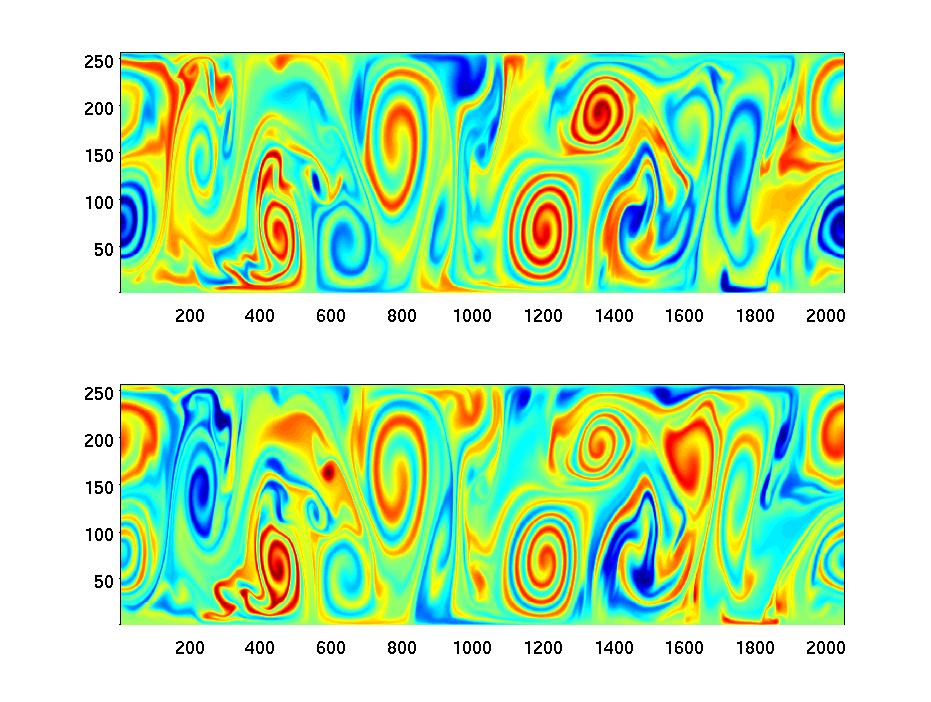
\includegraphics[width=0.85\textwidth]{111018t32_NL}
\\
(b)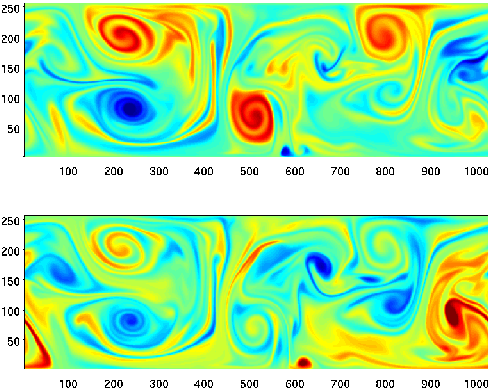
\includegraphics[width=0.85\textwidth]{111018reduced}
 }{}{
2 layers: top, bottom.
(a)
The usual domain $L=8$.
(b)
The reduced domain $L=4$, initial conditions starting
from a linear solution. The energy is not yet fully equilibrated.
The longer
cell (a) behaves pretty much the same way, but overall
the circulation is a bit stronger.
}{2layerBclin}
%%%%%%%%%%%%%%%%%%%%%%%%%%%%%%%%%%%%%%%%%%%%%%%%%%%%%%%%%%%%%%%%%%%%%

\begin{description}

\item[2011-05-27 Predrag, weather report from Snowbird DS11]
	\toCB
Learned from Pierrehumbert that the baroclinic models are to weathermen
what ``harmonic oscillator'' is to quantum mechanics. It has a continuous
East-West translational symmetry, \ie, in a periodic box it needs to be
sliced (the \SOn{2} of periodic box quotiented out).

Tried to proselytize Christian Wolfe\rf{WoSa07}, Scripts,  make him slice
the baroclinic instability, and, perchance, if I get him there, recycle
it, former Gibson style. Pierrehumbert says that this would be persuasive
to weather people, convince them to go looking for exact unstable
invariant solutions. After one hour Wolfe said he was converted.

Tried ditto with Pierrehumbert and Silber postdoc Yi-Ping Ma (Knobloch
trained, has worked with Spiegel at Woods Hole GFD). He does not know any
geophysical fluid dynamics yet, so I'm sceptical that he will do anything.

\item[2011-05-27 Annalisa Bracco]
If you ever need a code that produce baroclinic instability, I have
plenty. Worked with the Joe Pedlosky, the expert on Baroclinic
Instability, as a postdoc. I also have an easy atmospheric model (global,
on a sphere etc) that reproduces very well baroclinic instability as per
observations and can be run as aqua-planet to simplify things.

\item[2011-05-27 Predrag]
We could make Joe Pedlosky happy? Let's do it before August, in time for
Woods Hole. The first step is to slice your simulations for a minimal
periodic cell of interest (narrow but turbulent). The second step might
be either to determine ``physical dimension'' using
Wolfe-Samelson\rf{WoSa07} Lyapunov vectors (that is just simulation) or
find some traveling waves (that is Krylov-Arnoldi nontrivial work, but
for low-dimensional discretizations might be doable by Newton).

\item[2011-10-15 Annalisa]
Shown Predrag some simulations.
Each layer is computed in
terms of vorticity equations as a 2-dimensional fluid. The lower layer
has higher fluid density, and they are coupled across their interface by
difference of vorticity.
In our simulation this is about factor two; it is related to the
R\"osby deformation radius $L_R$. The spanwise $y$ width is $L_R/2\pi =
1/2$. Unless the width is larger than $L_R$, no instability. The
stream-wise aspect ration is about 8.
They tend to the barotropic solution (vortices rotating the same way on
top and bottom).


Discussion of solutions:
\begin{enumerate}
  \item [1)]
is linear: dropped the nonlinear term \ie\ the Jacobian of the vorticity
and the stream function. Instability is seeded by a small random field of
prescribed power spectrum, but the resulting instability is a localized
wave (about 3 rolls) with streamwise/spanwise ratio of about 1/2 set
$L_R$. That sets the scale of the instability off the laminar solution.
Initial noise does not matter, as the instability grows very fast. The
two layer vorticities are opposite.

  \item [2)] is fully nonlinear, all other parameters the same.

%  \item [3)]
\end{enumerate}

\item[2011-10-18 Annalisa]

\refFig{2layerBclin}\,(a)
The usual domain $L=8$, 2 layers. Note that as for initial conditions,
the overall the flow is more energetic.

\refFig{2layerBclin}\,(b)
The reduced domain $L=4$, 2 layers. Correct initial conditions, starting
from a linear solution. The energy is not yet fully equilibrated. One
problem I can see is that the periodic boundary conditions may prevent
perfect equilibration. The longer cell \refFig{2layerBclin}\,(a) behaves
pretty much the same way, but overall the circulation is a bit stronger.

\item[2011-10-19 Annalisa]
There is a barotropization issue, likely due to the periodic boundaries.
My guess is that we'll not need a very long simulation and we can live
with a non perfectly stationary state, essentially the eddies that form
in the equilibrated solution prefer to be barotropic -same sign top and
bottom layer- because they are more stable and in the absence of
viscosity they are an exact solution of \NS, and the simulation goes
into a state that resembles the long-term state for 2-d turbulence. If we
could work only over times $\sim $40-70 we should be all set.

For now the time is just in code units, I'll convert it in something
meaningful once we decide on which run to use, \etc.

%%%%%%%%%%%%%%%%%%%%%%%%%%%%%%%%%%%%%%%%%%%%%%%%%%%%%%%%%%%%%%%%%%%%%
\begin{figure}%[t]
\begin{center}
% \begin{tabular}{cc}
%        ~~~~~~~~(\textit{a})                        &   ~~~~~~~~(\textit{b}) \\
    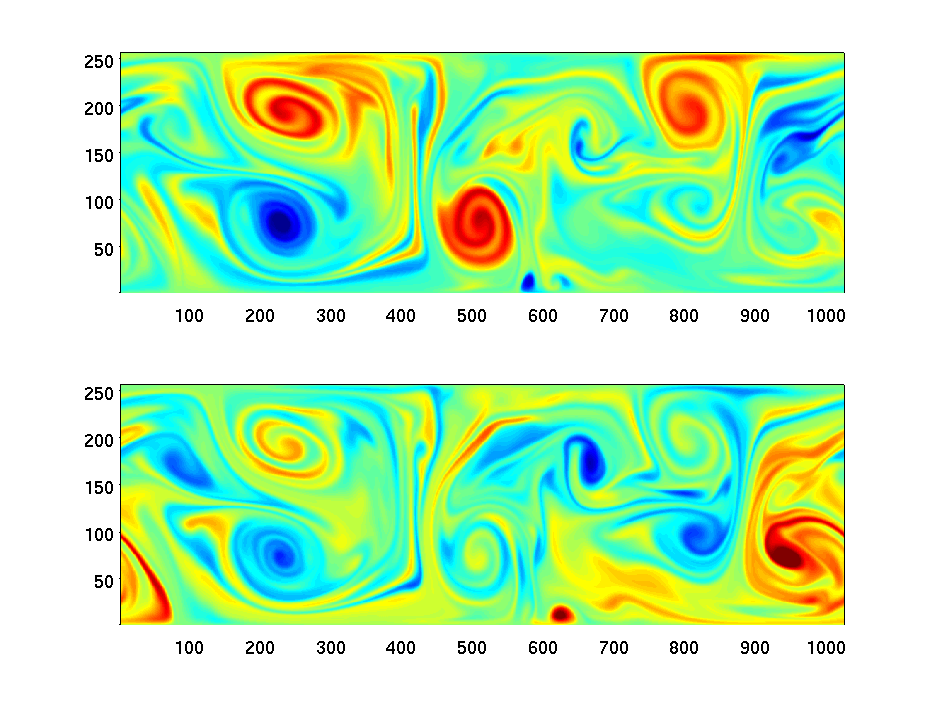
\includegraphics[width=0.85\textwidth]{111018time50}
%    &
    \\
    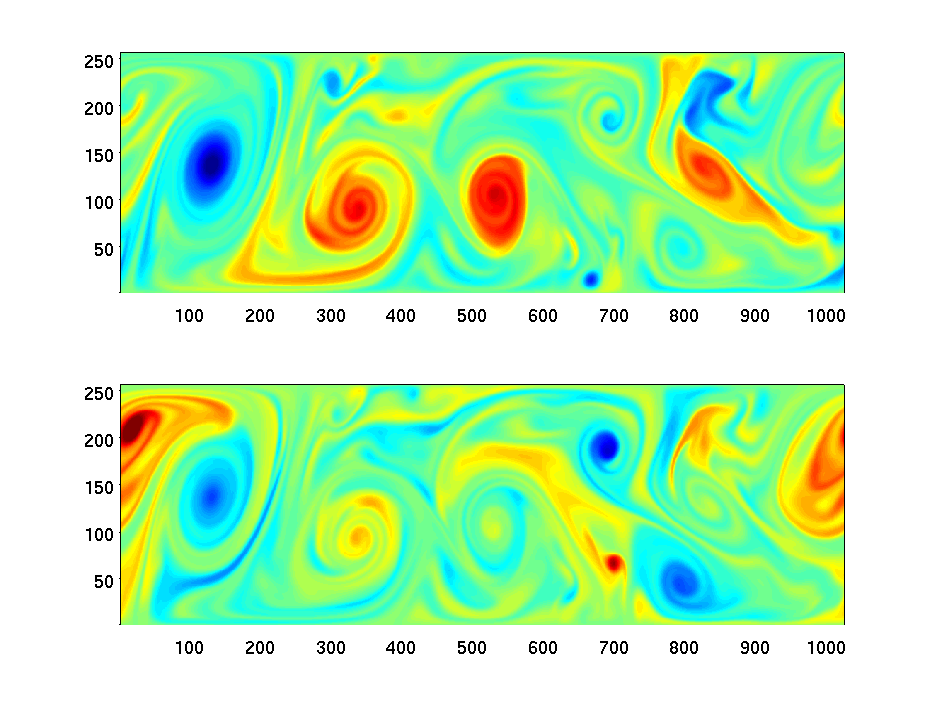
\includegraphics[width=0.85\textwidth]{111018time70}
%  \end{tabular}
\end{center}
\caption{
A plot of the vorticity in the top/bottom layers at times 50 and 70.
        }
\label{f:111018time1}
\end{figure}
%%%%%%%%%%%%%%%%%%%%%%%%%%%%%%%%%%%%%%%%%%%%%%%%%%%%%%%%%%%%%%%%%%%%%

%%%%%%%%%%%%%%%%%%%%%%%%%%%%%%%%%%%%%%%%%%%%%%%%%%%%%%%%%%%%%%%%%%%%%
\begin{figure}%[t]
\begin{center}
% \begin{tabular}{cc}
%        ~~~~~~~~(\textit{a})                        &   ~~~~~~~~(\textit{b}) \\
    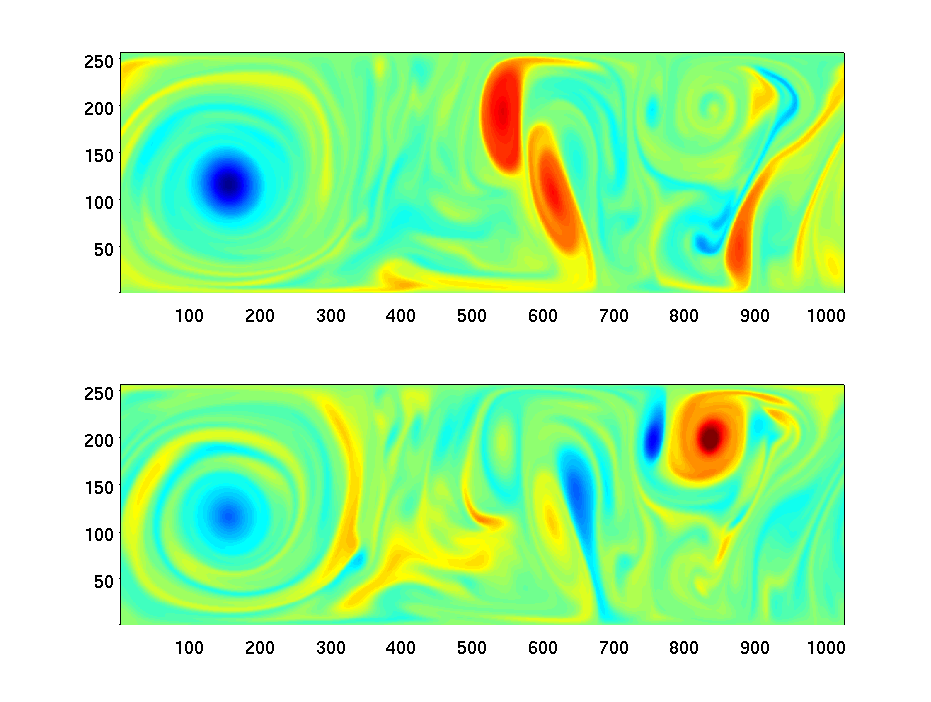
\includegraphics[width=0.95\textwidth]{111018time100}
%    &
%    \\
%    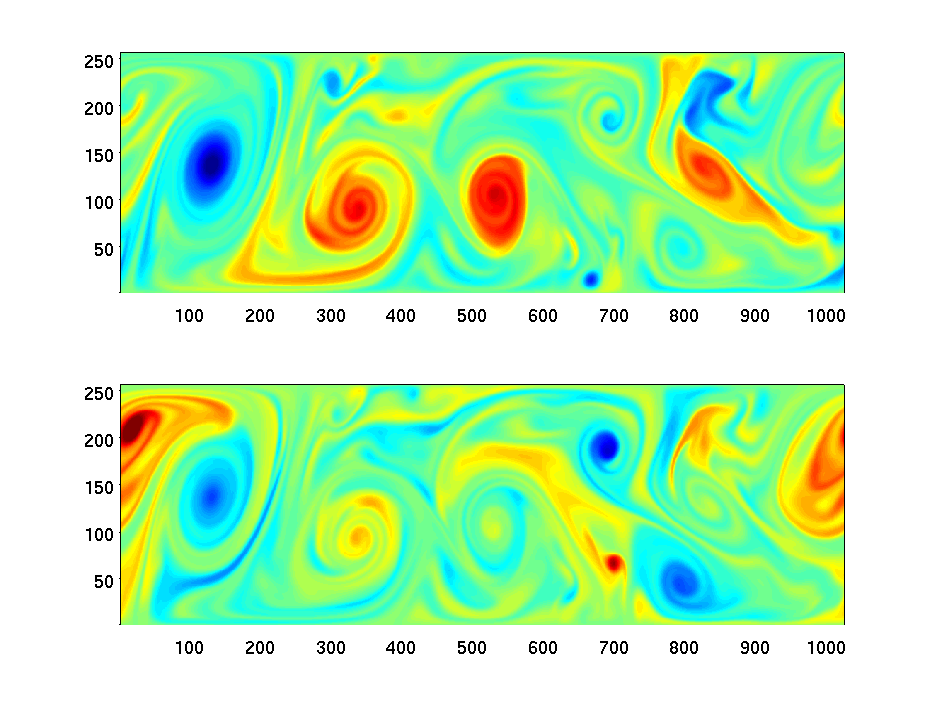
\includegraphics[width=0.95\textwidth]{111018time70}
%  \end{tabular}
\end{center}
\caption{
A plot of the vorticity in the top/bottom layers at time 100.
        }
\label{f:111018time2}
\end{figure}
%%%%%%%%%%%%%%%%%%%%%%%%%%%%%%%%%%%%%%%%%%%%%%%%%%%%%%%%%%%%%%%%%%%%%

%%%%%%%%%%%%%%%%%%%%%%%%%%%%%%%%%%%%%%%%%%%%%%%%%%%%%%%%%%%%%%%%%%%%%
\begin{figure}%[t]
\begin{center}
% \begin{tabular}{cc}
%        ~~~~~~~~(\textit{a})                        &   ~~~~~~~~(\textit{b}) \\
    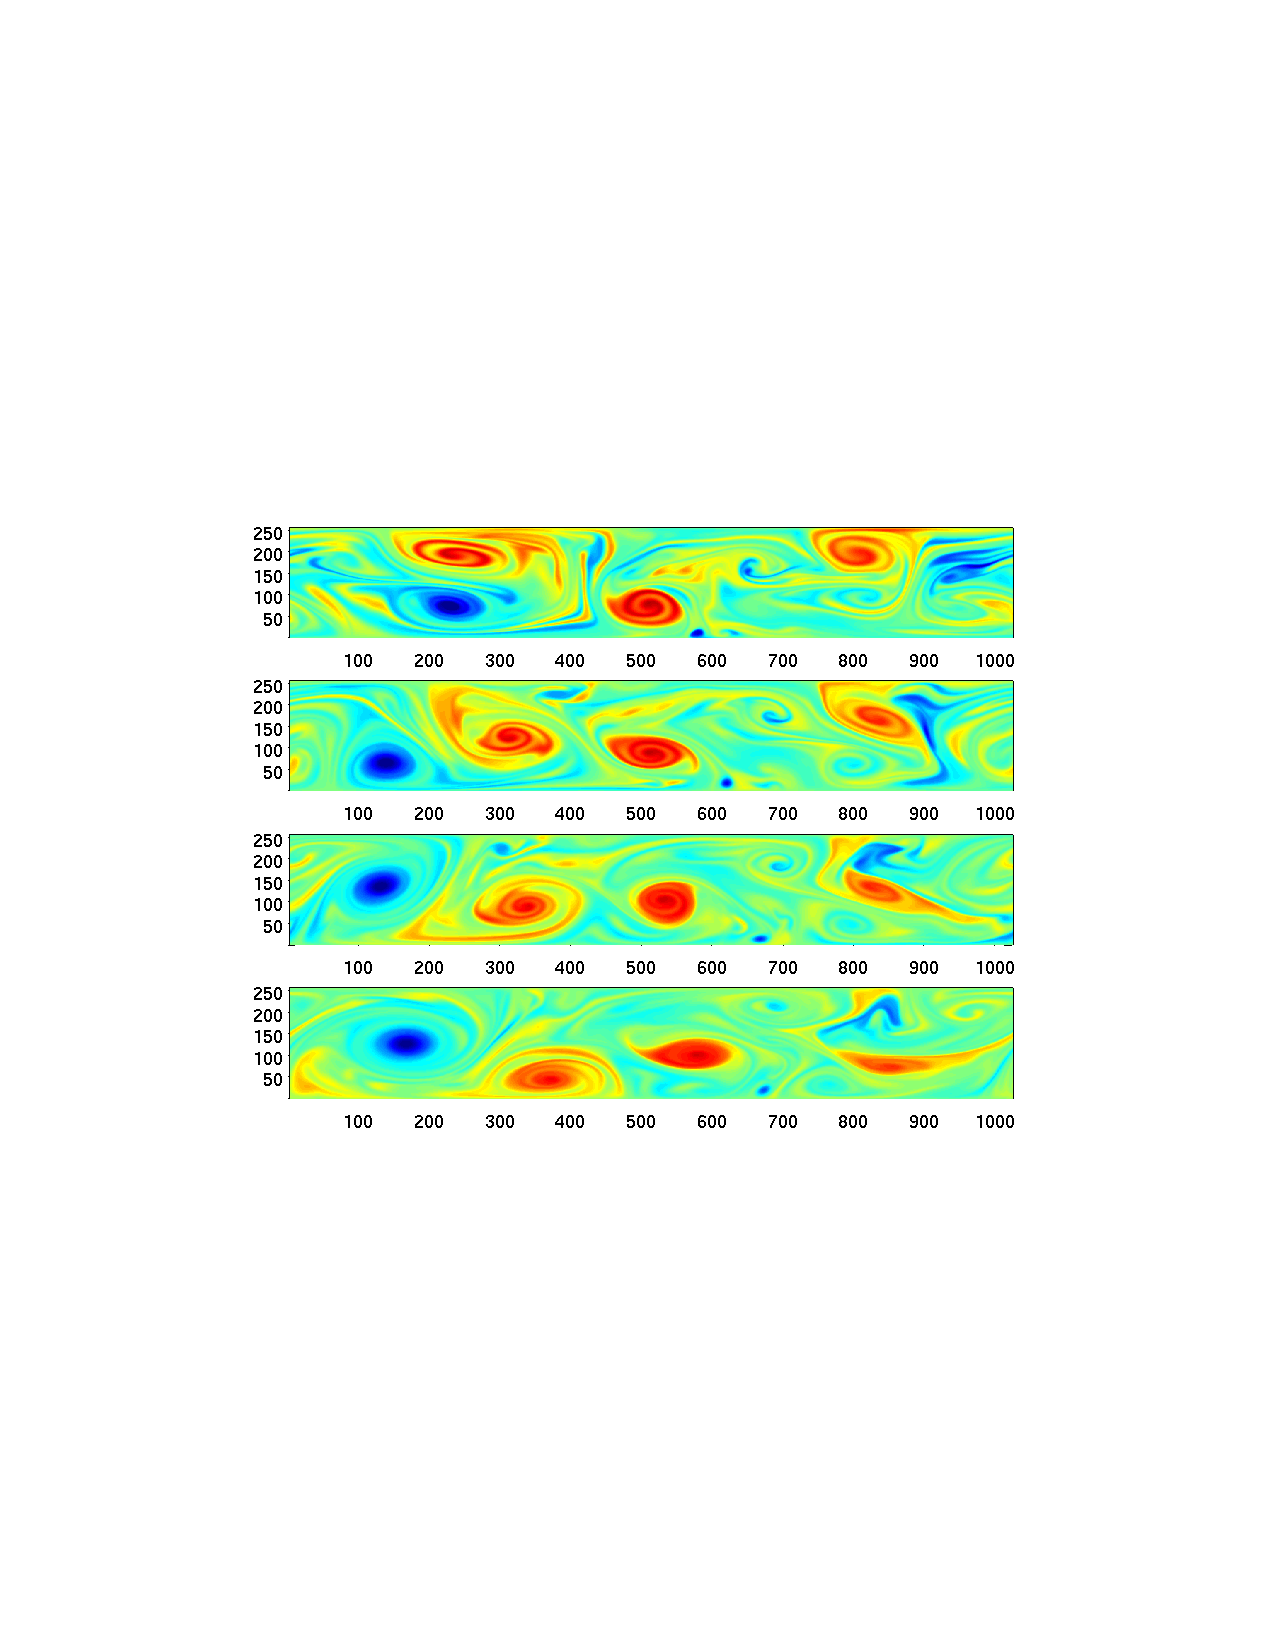
\includegraphics[width=0.95\textwidth]{111024layer1}
%    & 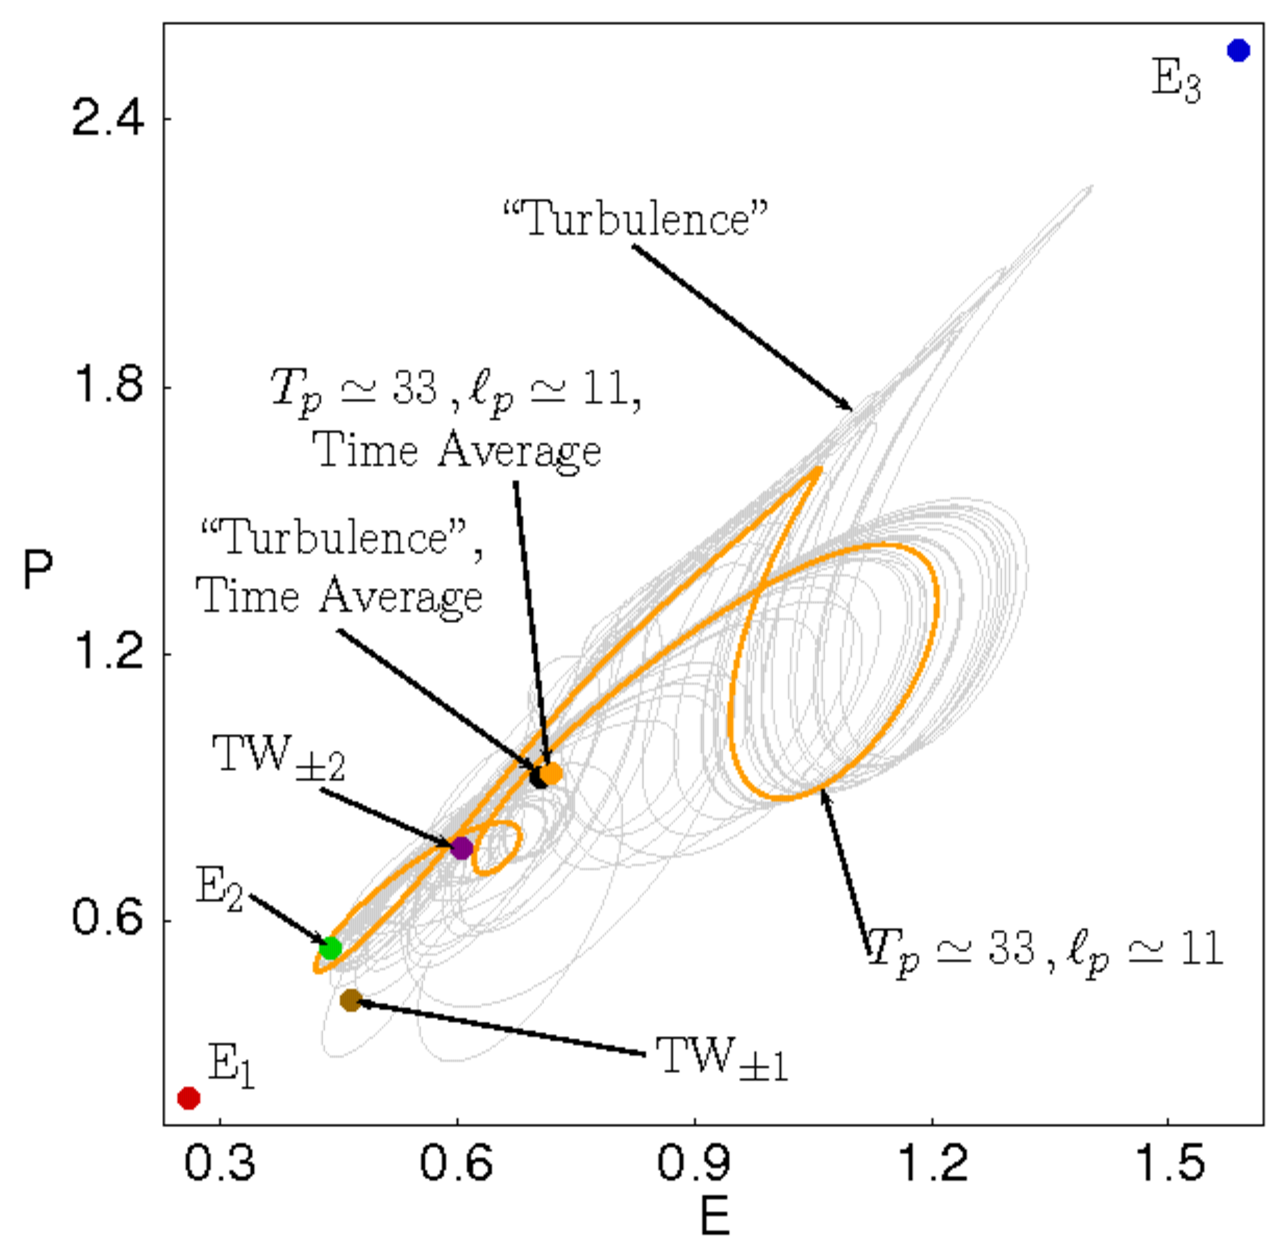
\includegraphics[width=0.46\textwidth, clip=true]{equivaEP_pst}
%  \end{tabular}
\end{center}
\caption{
A plot of the vorticity in the top layer at 4 different times during
which the energy is $\approx$ stable. The structures remain the same,
they are just moving a bit.
        }
\label{f:111024layer1}
\end{figure}
%%%%%%%%%%%%%%%%%%%%%%%%%%%%%%%%%%%%%%%%%%%%%%%%%%%%%%%%%%%%%%%%%%%%%



\item[2011-10-20 Predrag]
Bit worried if we are in transient turbulence, on the way to a
barotropic state, but might work out...

\item[2011-10-20 Annalisa]
One way to reduce the problem may be to stick to the 'longer' domain.
Another is to introduce a sponge region on one side. It will not solve the problem
completely: eddies are just more stable if barotropic and they tend to
become so while equilibrating a baroclinic solution, but it may delay
it.

\item[2011-10-20 Predrag]
It's OK that whole thing decays to barotropic, as long as we can find
unstable equilibrium solutions. Next (big) step. The short step is
to start looking at the dynamics of a short domain in the state space,
as explained in ChaosBook.org/tutorials, click on 'state space' in the
menu on the left.

\item[2011-10-20 Annalisa]
I may be able to stabilize it in a weakly nonlinear regime without
vortices but still something going on. I checked Wolfe PhD thesis and
it's all done in a very weakly nonlinear regime, so waves (just not
perfectly regular).

\item[2011-10-20 Edward A. Spiegel]
Baroclinic instability is a buoyancy driven instability in which
horizontal gradients and rotation play complicating parts.   Basically,
because of effect of rotation, the displacement of a fluid parcel that
unleashes the instability is not vertical as in R-B convection.  Or, if
you prefer, in the presence of rotation, your notion of what is vertical
is changed.

Pedlosky has written GFD lectures that do a pretty good job of explaining
the stuff.  If you are face to face with the right person, such as Joe,
it is no problem.  I think you should read a bit first and then talk to a
person. Anyway, it is time for you to test the waters of GFD books.  For
agreeable starts try Rick Salmon\rf{Salmon98} or James
Holton\rf{Holton79}.

Then talk to someone.

I once supervised a summer GFD project on baroclinic instability,
\HREF{http://www.whoi.edu/fileserver.do?id=21275&pt=10&p=17233}
{A. E. Hasha} (2005) report \emph{A Search for Baroclinic Structures}
and I think it made a nice self-contained package.
You may not want to start with that heavy a story.  I have some
easier stuff but I have no idea where you put it so I can say only
that you should look for the term ``Eady problem.''

\item[2011-10-20 Predrag 2 EAS]
Funny thing is I was reading Hasha when your email arrived. Nice report.
I can be more specific:

When I look at Annalisa's 2-layer simulations (driven at top by a
constant velocity field, streamwise length = 8 channel widths, Rossby
number = 2) it looks to me that baroclinic vortices get converted onto
barotropic ones, and there is nothing that would sustain generation of
new baroclinic vortices (opposite vorticity in the two layers), so there
is no sustained turbulence, it looks only transient. Or am I missing
something?

\item[2011-10-21 EAS]
This sounds like a case for cyclic behavior. If you keep running
Annalisa's case, I presume the barotropic vortices will run down and the
baroclinic instability will come back. That is, when the barotropic
vortices decay, you go back to the baroclinically unstable situation and
it all starts over.   Why it might do this instead of staying in a mildly
unstable, statistically steady case all the time is a bit of a mystery.
(Are you sure that it does not?)   There are other examples where systems
go cyclic in this way instead of maintaining a quasi-steady mean state
but I have not found the clue to predicting which case one will get.  For
example, why do things go all barotropic in your case?

\item[2011-10-21 Annalisa]
OK, but it'll take a LONG time, because the dissipation time of
relatively large, single eddies is pretty small. This is one of those
situations where the model domain plays such a role that the 'real'
application is close to null.

\item[2011-10-22 Predrag 2 Annalisa] I'm working on writing up
the physical ways of projecting turbulent flows onto handful of
\statesp\ coordinates. The derivation of the first set,
$(E(\zeit),D(\zeit),I(\zeit))$ and generalizations is illustrated by
a simpler case, the \KSe, in \refsect{sec:moreObs}. I'll try to get to
the \NS\ case and the much better Gibson et al. coordinates, but it
is taking time...

\item[2011-10-24 Annalisa]
Still not convinced about the flow field per se. \refFig{f:111018time1}
and
\refFig{f:111018time2}
are plots of the vorticity in the top layer at 3 different times during
which the energy is $\approx$ stable (at least the kinetic part, but
being dominant also the total is OK). The problem is that the structures I
see are always the same, they are just moving a bit. And this is going to
be the case with this channel once is equilibrated.

BTW, Lo Specchio  is theoretically right, but practically wrong.
Barotropic vortices can take a long time to dissipate. By that time,
everything else dissipated as well (\ie, any residual perturbation of the
flow field) and there is nothing on which the baroclinic instability will
be able to feed upon: if you start with zero perturbation field in the
Phillips model, you'll still end up with zero perturbation everywhere.

\item[2011-10-20 Predrag] I understand - they are sort of frozen in. In
spatiotemporal chaos it is one of the possible phases of an extended
system, but for weathermen, this is no fun at all. There must be
something to baroclinic instability that I am missing - it cannot be that it
is just a complicated transient? In that case we might have to drive it
by noisy surface winds, but that will be harder...

\item[2011-10-24 Annalisa]
My take on baroclinic instability: wonderful linear theory. Practically
useful only to figure out where you form eddies. I can still try to
reduce further the dimension of the domain and see what happens in that
case...

\item[2011-10-20 Predrag] Something quite different but of interest to me;
the reason you always see spirals in these $N$-layer models is that locally
$2D$ fluid mechanics is Euclidean-invariant? In a full $3D$ simulation these
vortices would still be there because of horizontal layers of fluid of equal density?

\item[2011-10-24 Annalisa]
Personal take on the spirals... It looks that is the best way for the
eddies to barotropize. There must be some energy conversion mechanism
that favors them.

\item[2011-10-24 Annalisa]
The physics of 2d turbulence is .. 2d turbulence. It creates vortices.
More relevant for the ocean than the atmosphere, but baroclinic
instability creates vortices as well.

\item[2011-10-25 Annalisa, Predrag, Joe Pedlosky] (conference call,
Joe office 508-289-2534, home 508-548-2069;
Annalisa cell 404-323-7722, office 404-323-7722, home 404-724-0975;
Predrag 404-IT-STINX everywhere)

\noindent{\bf Annalisa} I'm running 2-layer Phillips model, driven by fixed velocity at
the surface, bottom layer is at rest. Use $\beta=0$; tried with $\beta
\neq 0$, but it makes no difference. In linear solution, instability
kicks in, goes unstable linearly \emph{very} fast. In nonlinear regime it
does not get into equilibrated state, nonlinear term wants to generate
spirals which then drive the flow into barotropic state.

\noindent{\bf Joe} What maintains the flow?

\noindent{\bf Annalisa} Specifying initial zonal velocity - maintain
constant current on the top layer, always there. Friction is Newtonian
viscosity in both layers. Deformation radius (PC: Rossby number?) is such
that the channel is twice that. I tried with 4 times the radius, nothing
changes.

\noindent{\bf Joe} Even though is baroclinicity is maintained by constant surface
drive? Flat 2-layer model requires $F = $(wavenumber)$^2/2\pi \approx 5$,
a fairly large number. In your setup baroclinic instability is maybe not
driving. In our simulations we get baroclinic
production everywhere in the bulk for $F \approx 4$.

What if viscosity only in the bottom layer?

\noindent{\bf Annalisa} In literature I never saw equilibrated 2-layer Phillips.

\noindent{\bf Joe} A man called P, but not me, from Texas A\& M had a number of
simulations, looking for equilibrated state. The references are
Panetta\rf{PaHe88,Panetta93} and Pedlosky\rf{KlPe86}

Predrag: alert me if we should read any of the related
\refrefs{HePaPi85,HePiPa86,PaHePi87,ZePiEy93}, or
\refrefs{HeLa96,MoSiSo07,HoWi05,WeHa89,Mak87,RiKl97,
Shepherd88,Young87,PeKl91,KlPe92,WeBa88,PePo87}.

\item[2011-10-26 Annalisa]
I read the papers Joe' suggested. Two have no vortices (the 1d
Panetta\rf{PaHe88} and the one by Joe\rf{KlPe86}). The
Panetta\rf{Panetta93} may be relevant but very limited resolution (so
vortices may not form in that case as well. Hard to say from just
streamfunction plots). Still Panetta does reach an equilibrium state.
Set-up pretty similar (except for periodic conditions). I wrote exactly
that code, but in 2000, and I don't have a copy (lost somewhere in
Torino). Not sure when I can re-write it from scratch if necessary (need
really to write a paper first).

Alert Joe that the figures are at the end of this text (I can also make
plots of the energy in time). The equations need some correction.

\item[2011-10-26 Joe]
Thanks for the creature from the Blog Lagoon?. I have really
one very simple question that I could not find in the write-up.

What is the width you use to scale the horizontal lengths? Or, more
specifically, what is the ratio of the width of the channel to the
deformation radius? I am trying to see what the value of the parameter
\[
F= (f^2L^2)/g'H
\]
is in your calculations where $H$ is the depth of each layer and $L$ is
the channel width.

\item[2011-10-26 Annalisa]
I tried with different sizes, but always in what should be an unstable
regime according to the Phillips criteria and our old calculations with
the same code (and it always is unstable in the linear case). I modified
all the numbers twice since the simulation shown in the notes, so I'm not
100\% sure (anyway, that run is useless), but I usually set $F= 1$ 'model
unit'  and the width of the channel has been varied between $\pi$ and
$2\pi$  ($4\pi$  as for yesterday and still nothing). Starting to think I
may have made a mistake somewhere while removing the topography term from
the old code and somehow I'm not getting the upper current in the
non-linear calculations, because it makes no sense.

%%%%%%%%%%%%%%%%%%%%%%%%%%%%%%%%%%%%%%%%%%%%%%%%%%%%%%%%%%%%%%%%%%%%%
\begin{figure}%[t]
\begin{center}
% \begin{tabular}{cc}
%        ~~~~~~~~(\textit{a})                        &   ~~~~~~~~(\textit{b}) \\
    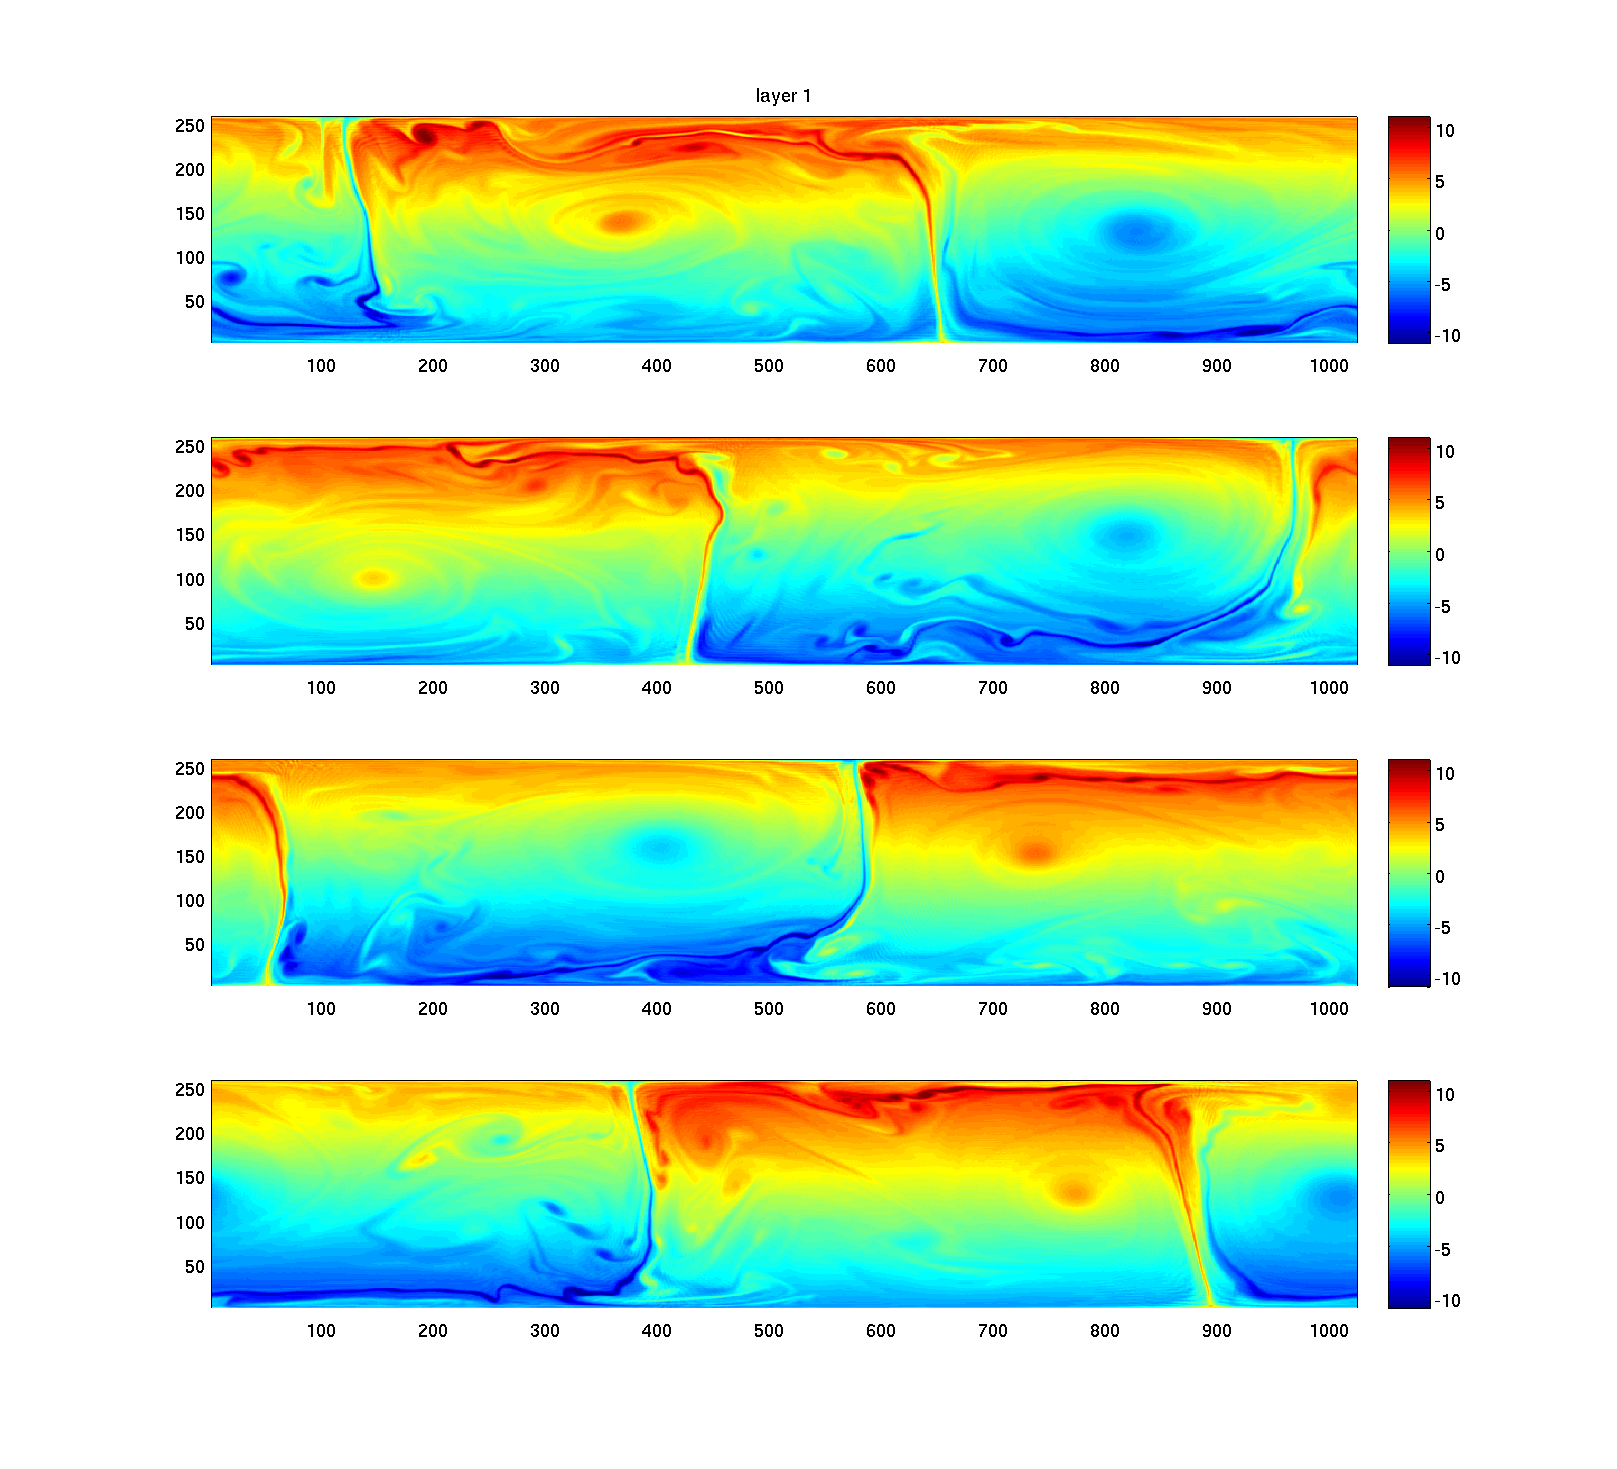
\includegraphics[width=0.95\textwidth]{111028layer1}
%    & 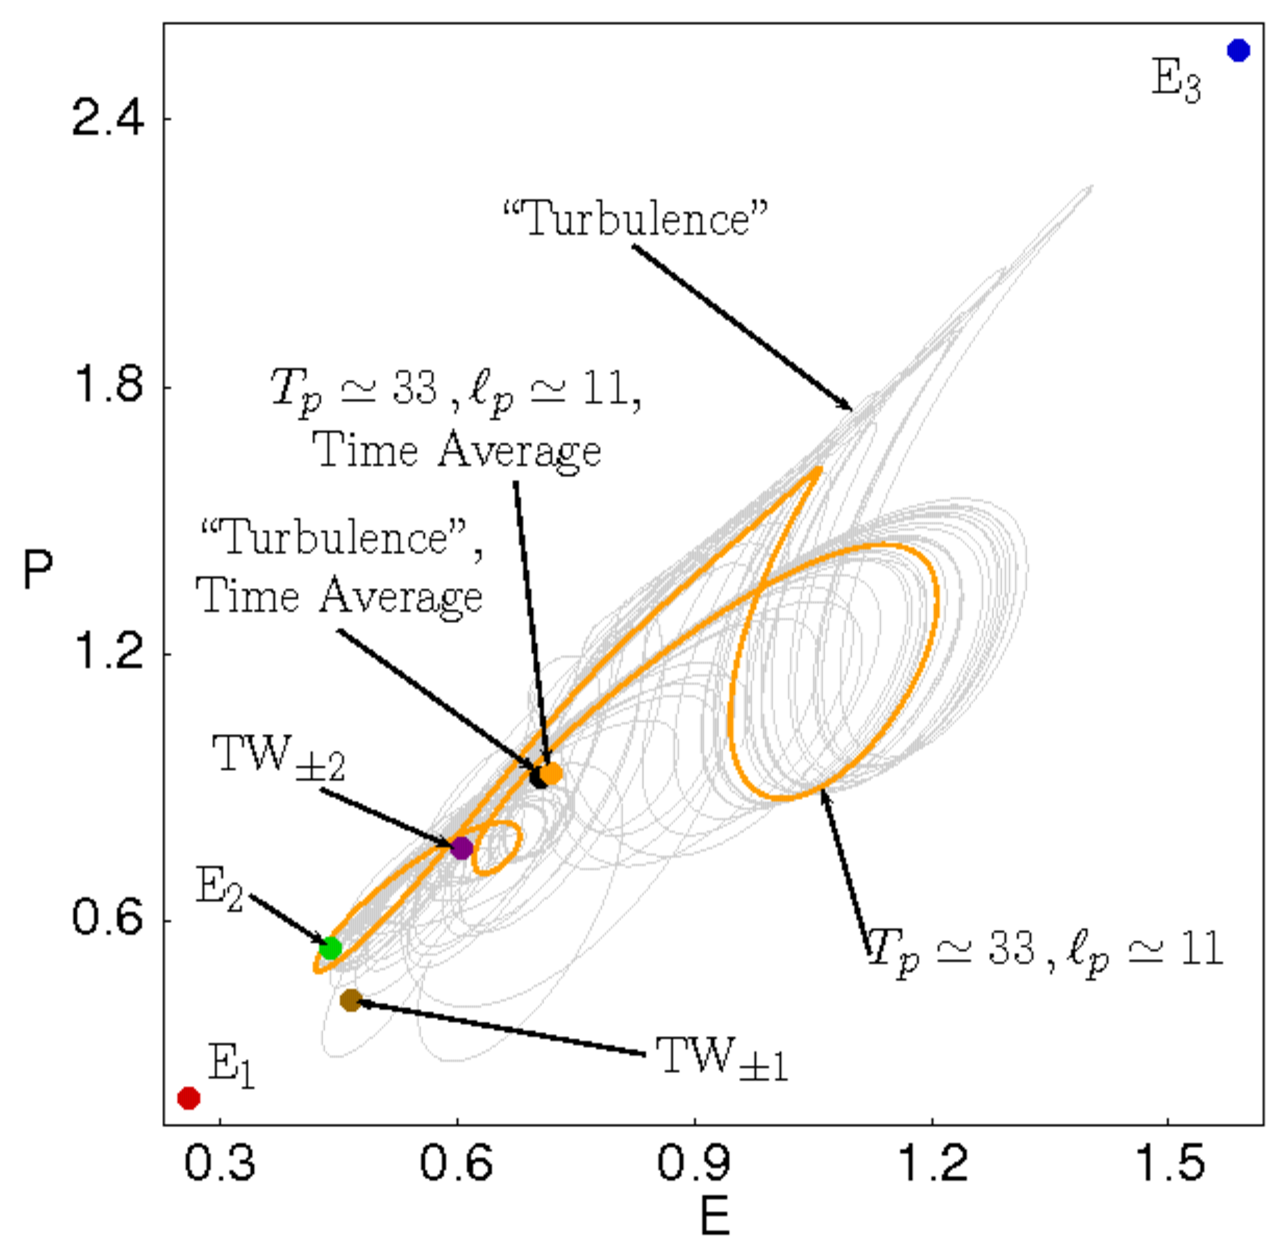
\includegraphics[width=0.46\textwidth, clip=true]{equivaEP_pst}
%  \end{tabular}
\end{center}
\caption{
The top-layer fixing term now corrected (all previous figures are wrong).
A plot of the vorticity in the top layer at 4 different times, but energy
is still increasing, see \reffig{f:111028energy}.
        }
\label{f:111028layer1}
\end{figure}
%%%%%%%%%%%%%%%%%%%%%%%%%%%%%%%%%%%%%%%%%%%%%%%%%%%%%%%%%%%%%%%%%%%%%

%%%%%%%%%%%%%%%%%%%%%%%%%%%%%%%%%%%%%%%%%%%%%%%%%%%%%%%%%%%%%%%%%%%%%
\SFIG{111028energy}
{}{
The kinetic energy for the evolution of \reffig{f:111028layer1}. To
Predrag the top curve looks monotonically increasing (energy cannot do
that, and the pictures of flow do not look like they are speeding up) and
he has no idea what the bottom curve is.
}{f:111028energy}
%%%%%%%%%%%%%%%%%%%%%%%%%%%%%%%%%%%%%%%%%%%%%%%%%%%%%%%%%%%%%%%%%%%%%

\item[2011-10-28 Annalisa]
Fixed the bug in the top layer driving term, see \reffig{f:111028layer1}.
The kinetic energy \reffig{f:111028energy} is still growing, but the
potential is stable. I'll play with the dissipation. There is still a
tendency for the eddies to barotropize (no reason that should change), so
not sure if the kinetic energy will ever get perfectly stable (unless I
dissipate a lot).

\item[2011-10-28 Predrag] Talked to John Gibson, Skype johnfgibson. He
thinks it would be easiest to append his Newton-Krylov-Arnoldi solvers to
your code - you guys can talk about it.

\item[2011-10-28 Annalisa]
You seem to have an automatic forward to some gmail account with a
limited size allowed If you wish to look at the second one, let me know
and I'll send it separately.

\item[2011-10-28 Predrag] You are using Mac at work, or Linux, or?

\item[2011-11-09 Annalisa]
\refFig{f:111109layer} is a run with much lower (10 times lower) large
scale dissipation. Not perfectly equilibrated though, see
\reffig{f:111109kin-pot}. %\,(a) \reffig{f:111109kin-pot}\,(b)

I'll remove the dissipation at large scale in the top layer, convert the
operator into Ekman and see if I can get a stationary state if you think
is still worth it.


%%%%%%%%%%%%%%%%%%%%%%%%%%%%%%%%%%%%%%%%%%%%%%%%%%%%%%%%%%%%%%%%%%%%%
\begin{figure}%[t]
\begin{center}
 \begin{tabular}{cc}
        ~~~~~~~~(\textit{a})                        &   ~~~~~~~~(\textit{b}) \\
    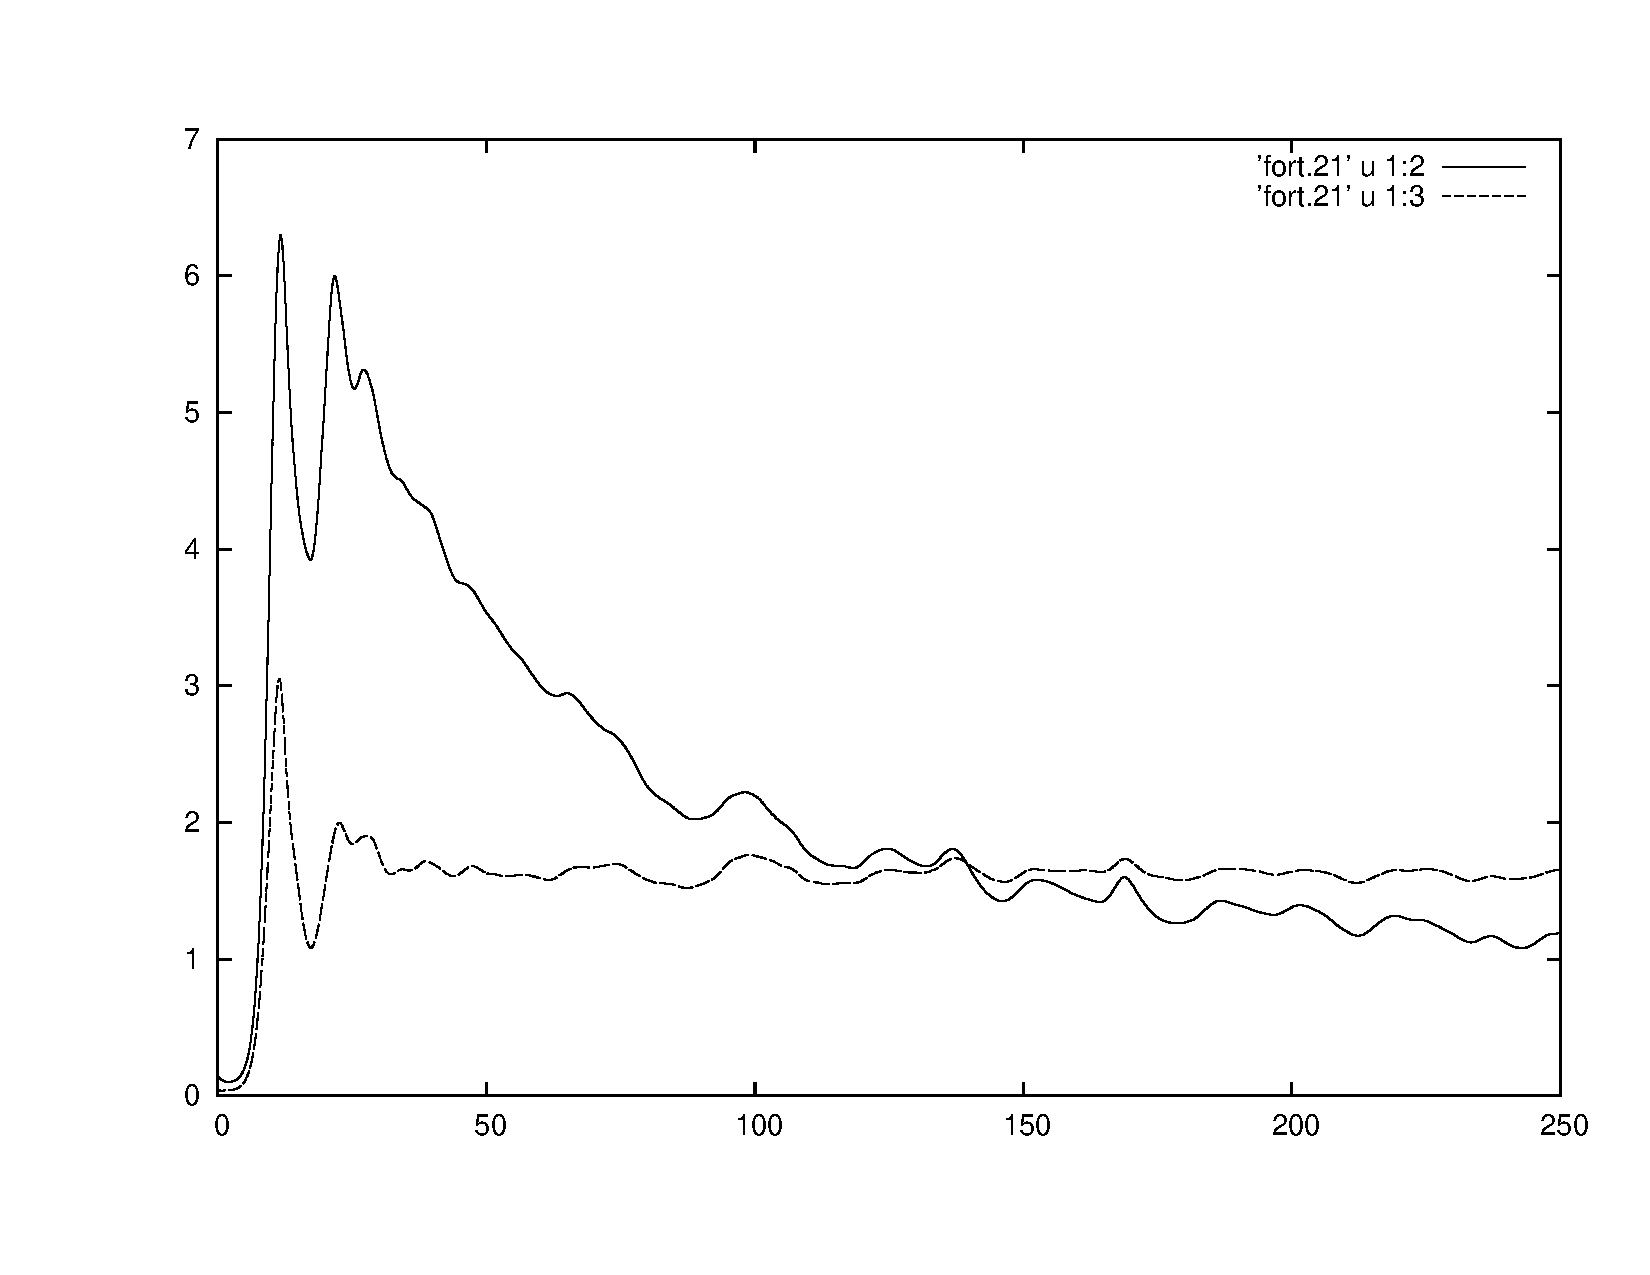
\includegraphics[width=0.45\textwidth]{111109ene}
    &
    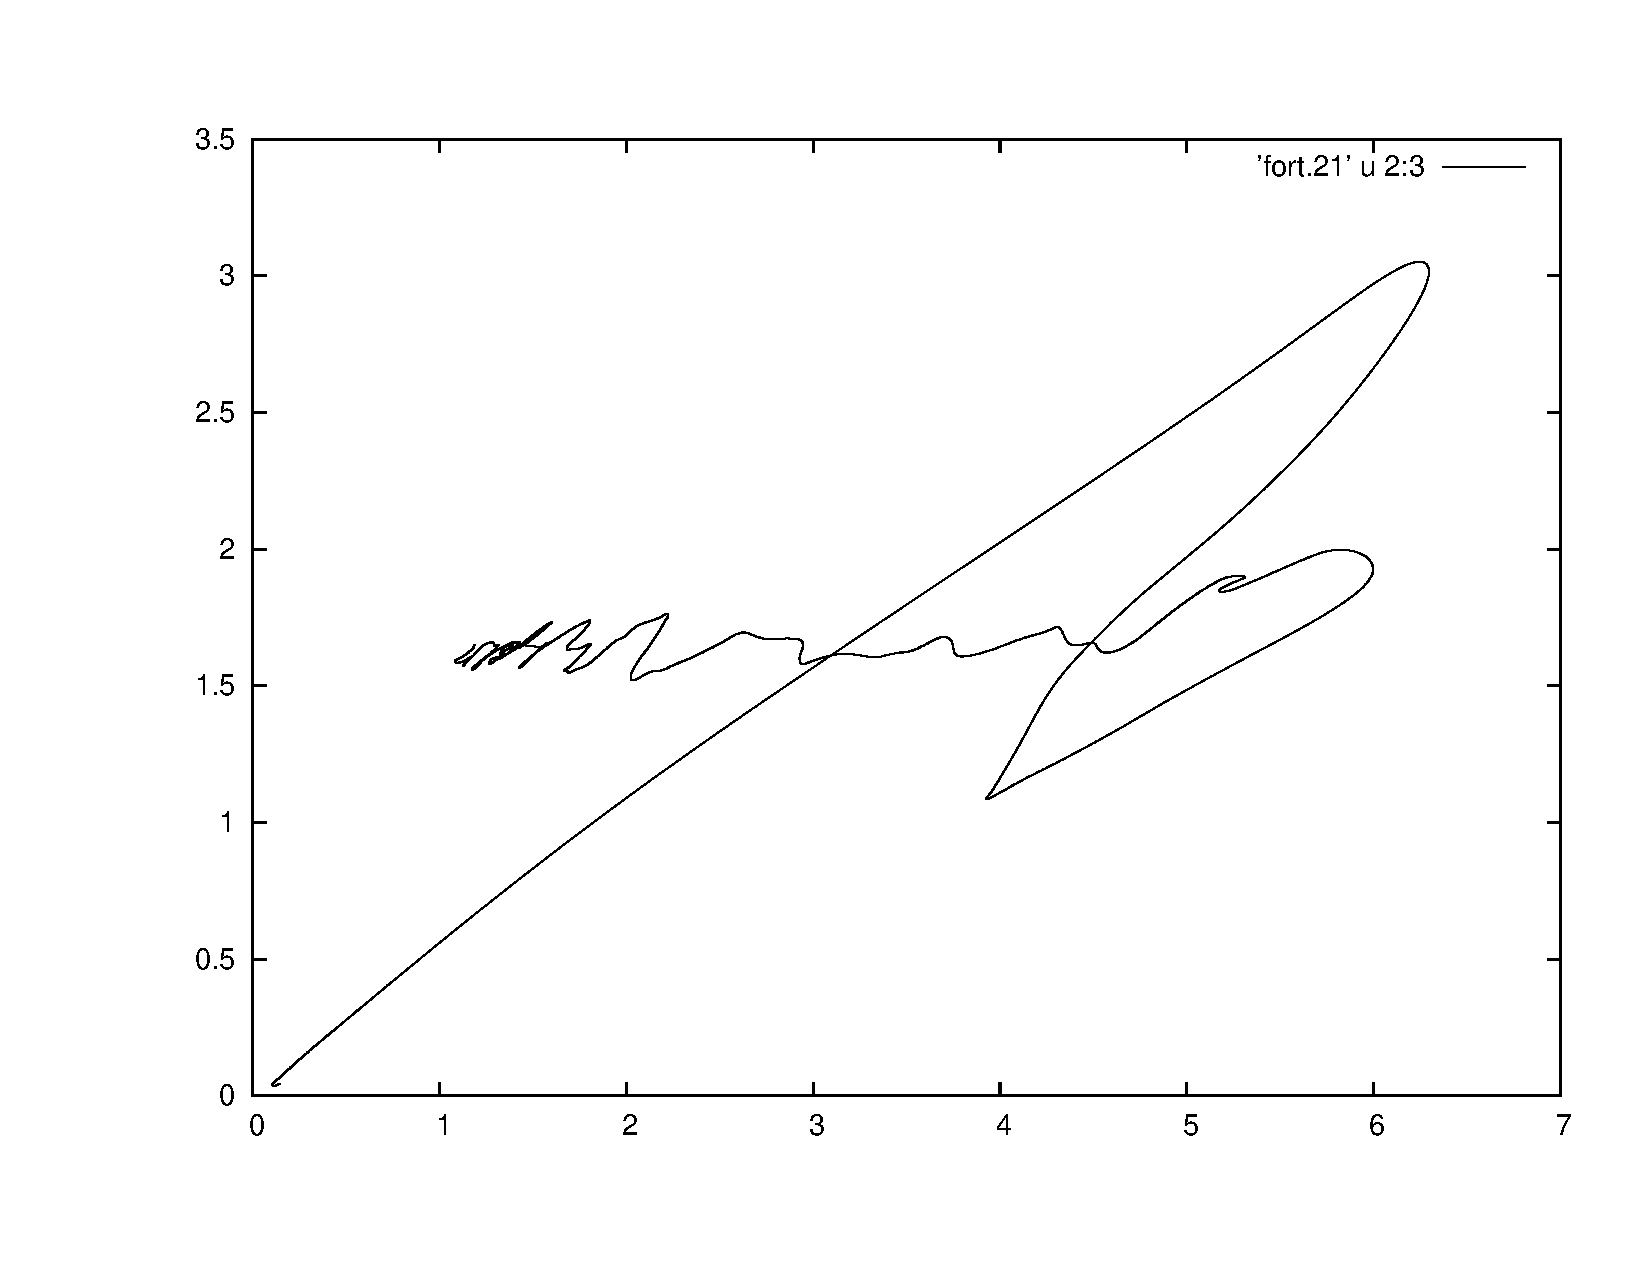
\includegraphics[width=0.45\textwidth]{111109kin-pot}
  \end{tabular}
\end{center}
\caption{
The kinetic and potential {\em vs} kinetic energy plots
for the evolution of \reffig{f:111109layer}.
        }
\label{f:111109kin-pot}
\end{figure}
%%%%%%%%%%%%%%%%%%%%%%%%%%%%%%%%%%%%%%%%%%%%%%%%%%%%%%%%%%%%%%%%%%%%%

%%%%%%%%%%%%%%%%%%%%%%%%%%%%%%%%%%%%%%%%%%%%%%%%%%%%%%%%%%%%%%%%%%%%%
\begin{figure}%[t]
\begin{center}
% \begin{tabular}{cc}
%        ~~~~~~~~(\textit{a})                        &   ~~~~~~~~(\textit{b}) \\
    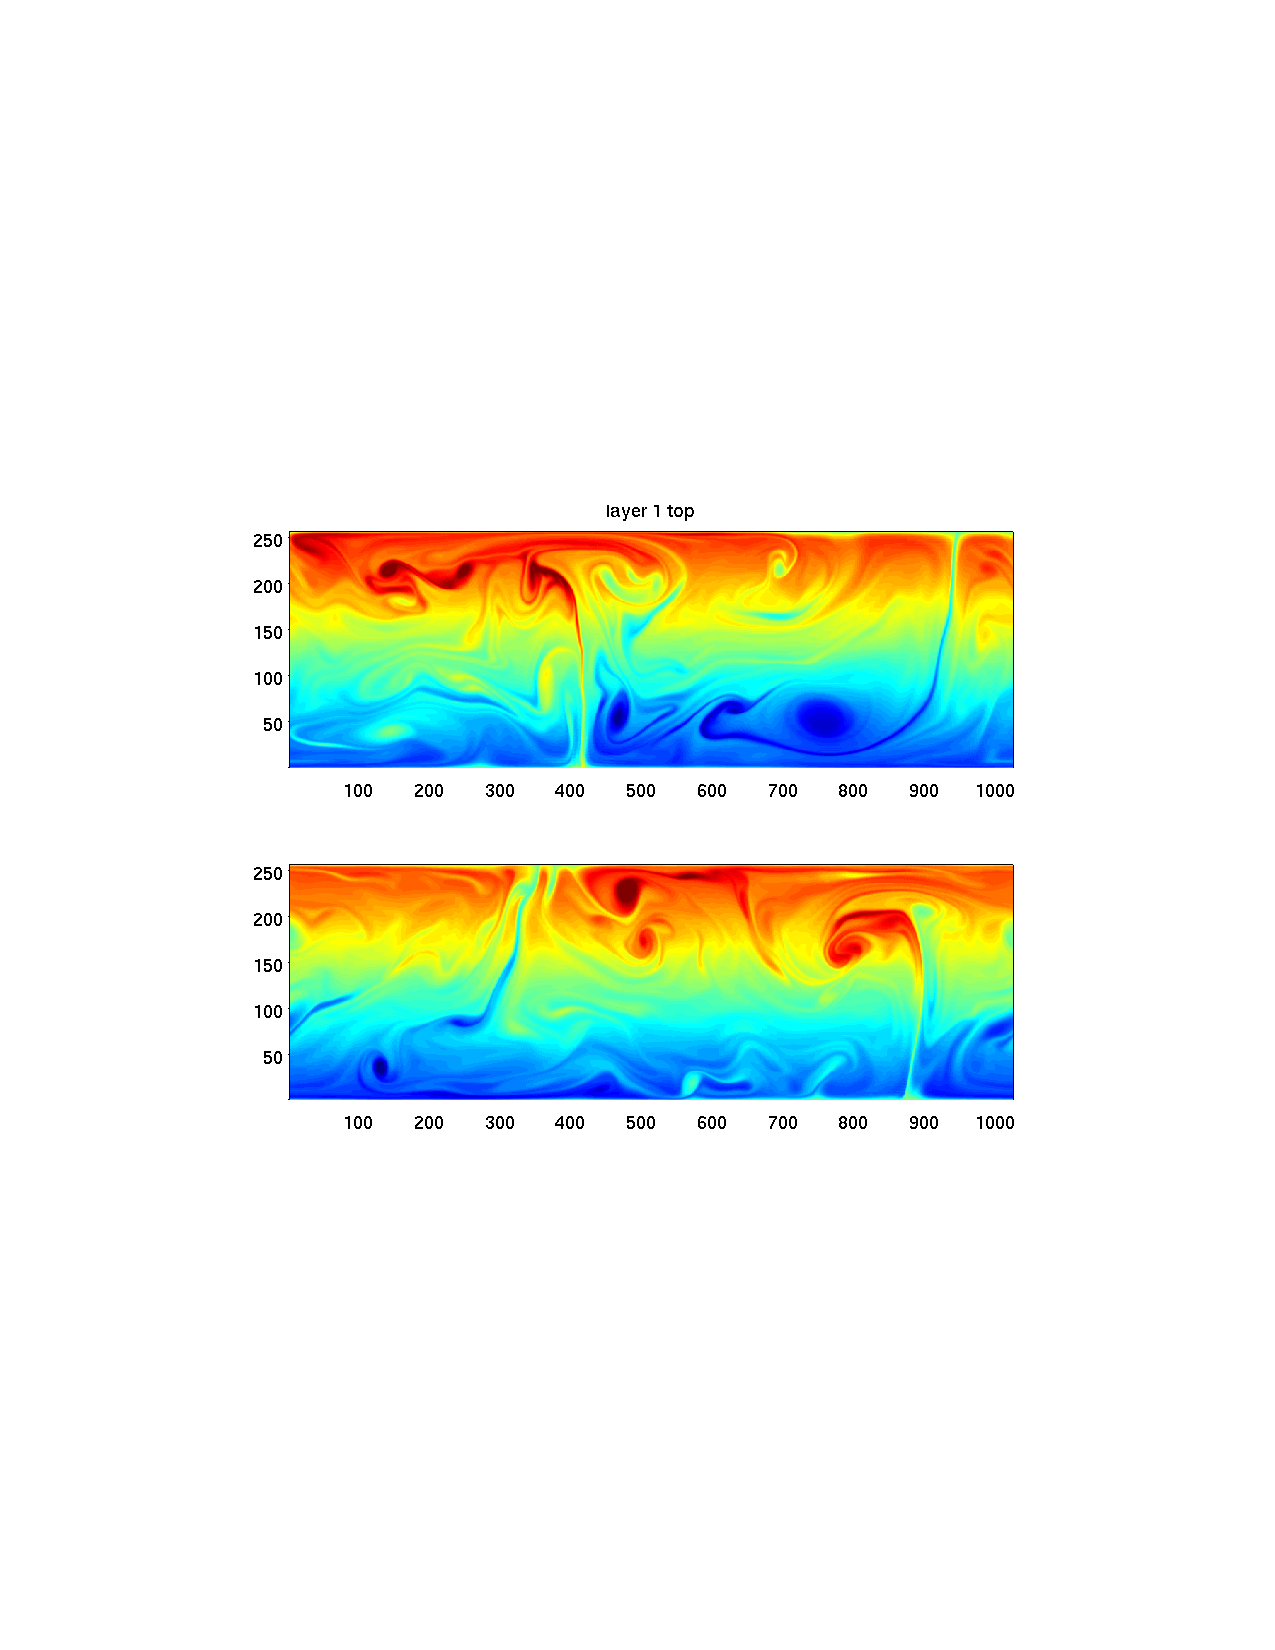
\includegraphics[width=0.85\textwidth]{111109layer1}
%    &
    \\
    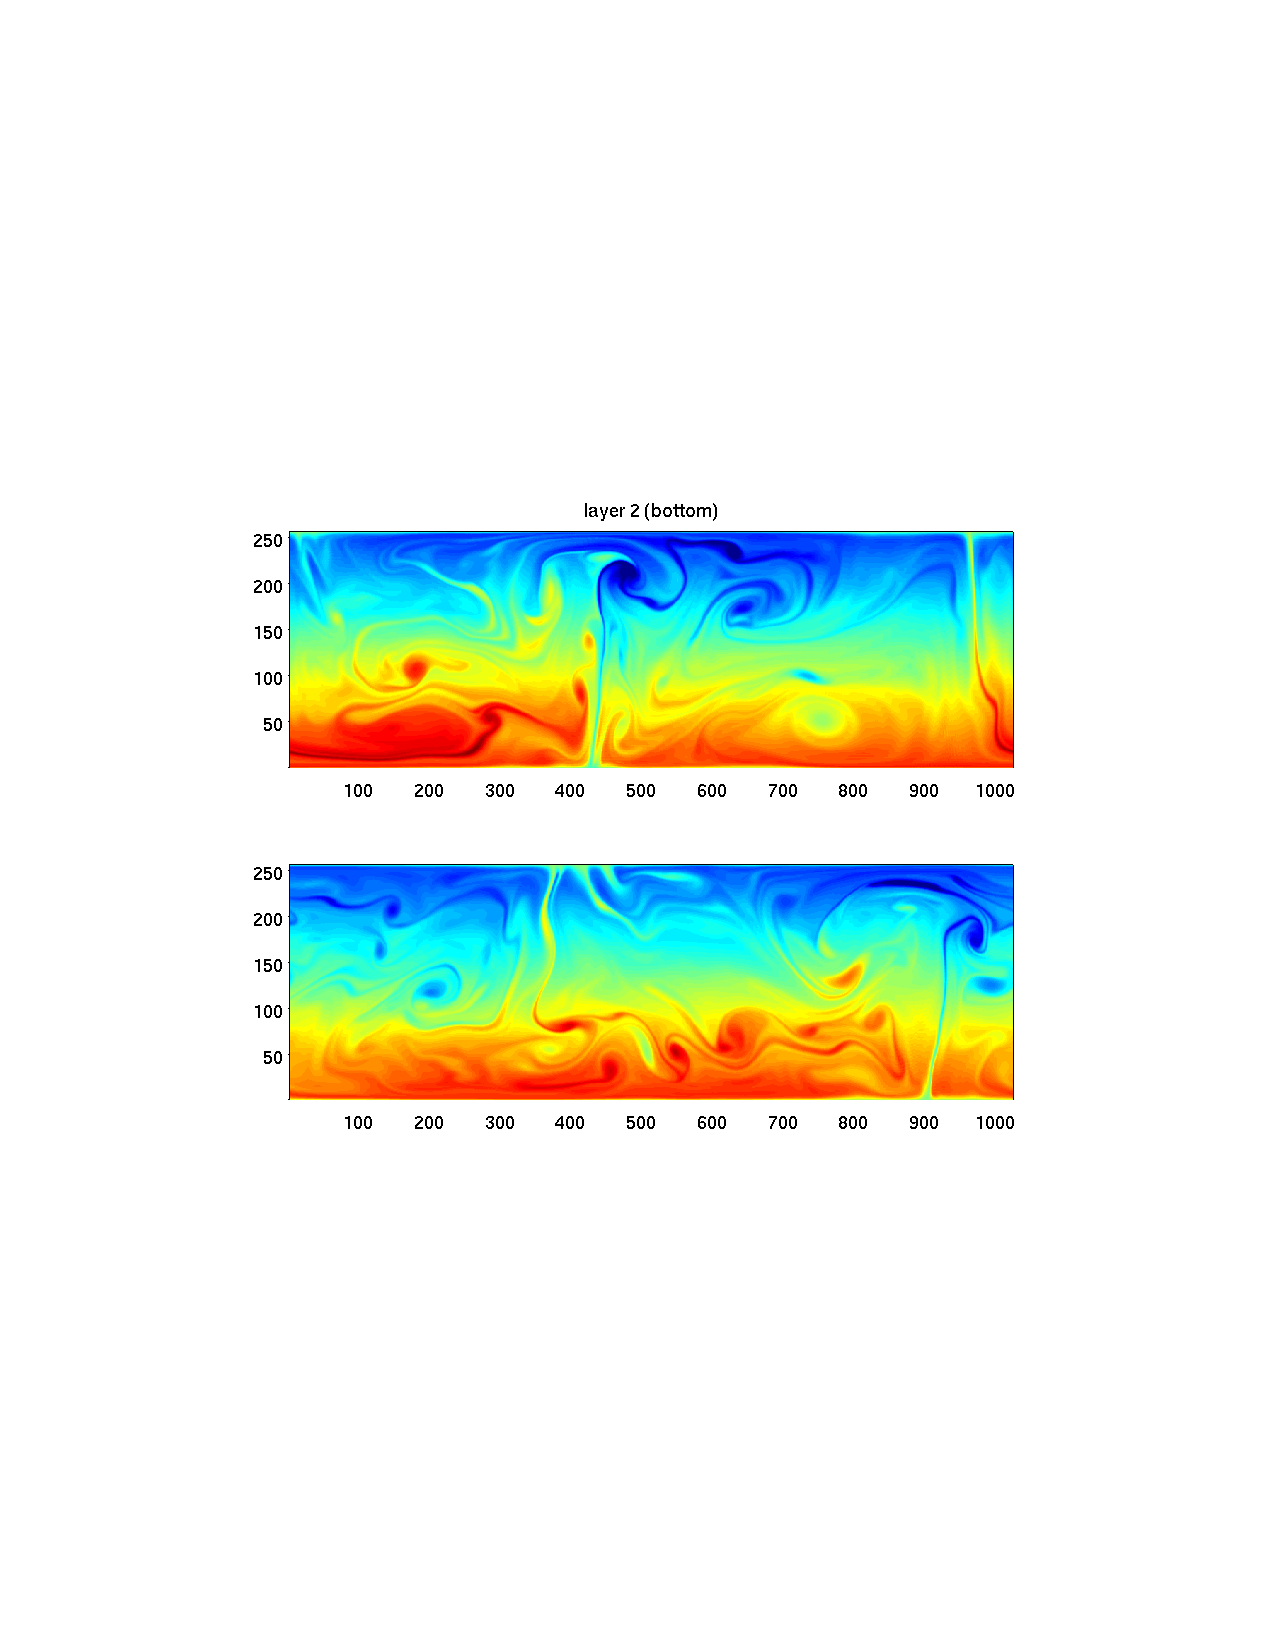
\includegraphics[width=0.85\textwidth]{111109layer2}
%  \end{tabular}
\end{center}
\caption{
A plot of the vorticity in the top/bottom layers at times ?0 and ?0.
        }
\label{f:111109layer}
\end{figure}
%%%%%%%%%%%%%%%%%%%%%%%%%%%%%%%%%%%%%%%%%%%%%%%%%%%%%%%%%%%%%%%%%%%%%

\item[2011-11-09 Predrag] The plots are pretty. I think removing the
dissipation at large scale from the top layer, and converting the
operator into Ekman would be more physical. If you can get a stationary
state we could at least use it for motivational purposes for the AGU
meeting.

I'm worried about plotting potential vs kinetic energy - their sum might
be approximately conserved, masking turbulent dynamics. It would be
better if you can plot the rates such as power in, dissipation out in
\refeq{Power=I-D}.

%%%%%%%%%%%%%%%%%%%%%%%%%%%%%%%%%%%%%%%%%%%%%%%%%%%%%%%%%%%%%%%%%%%%%
\begin{figure}%[t]
\begin{center}
% \begin{tabular}{cc}
%        ~~~~~~~~(\textit{a})                        &   ~~~~~~~~(\textit{b}) \\
    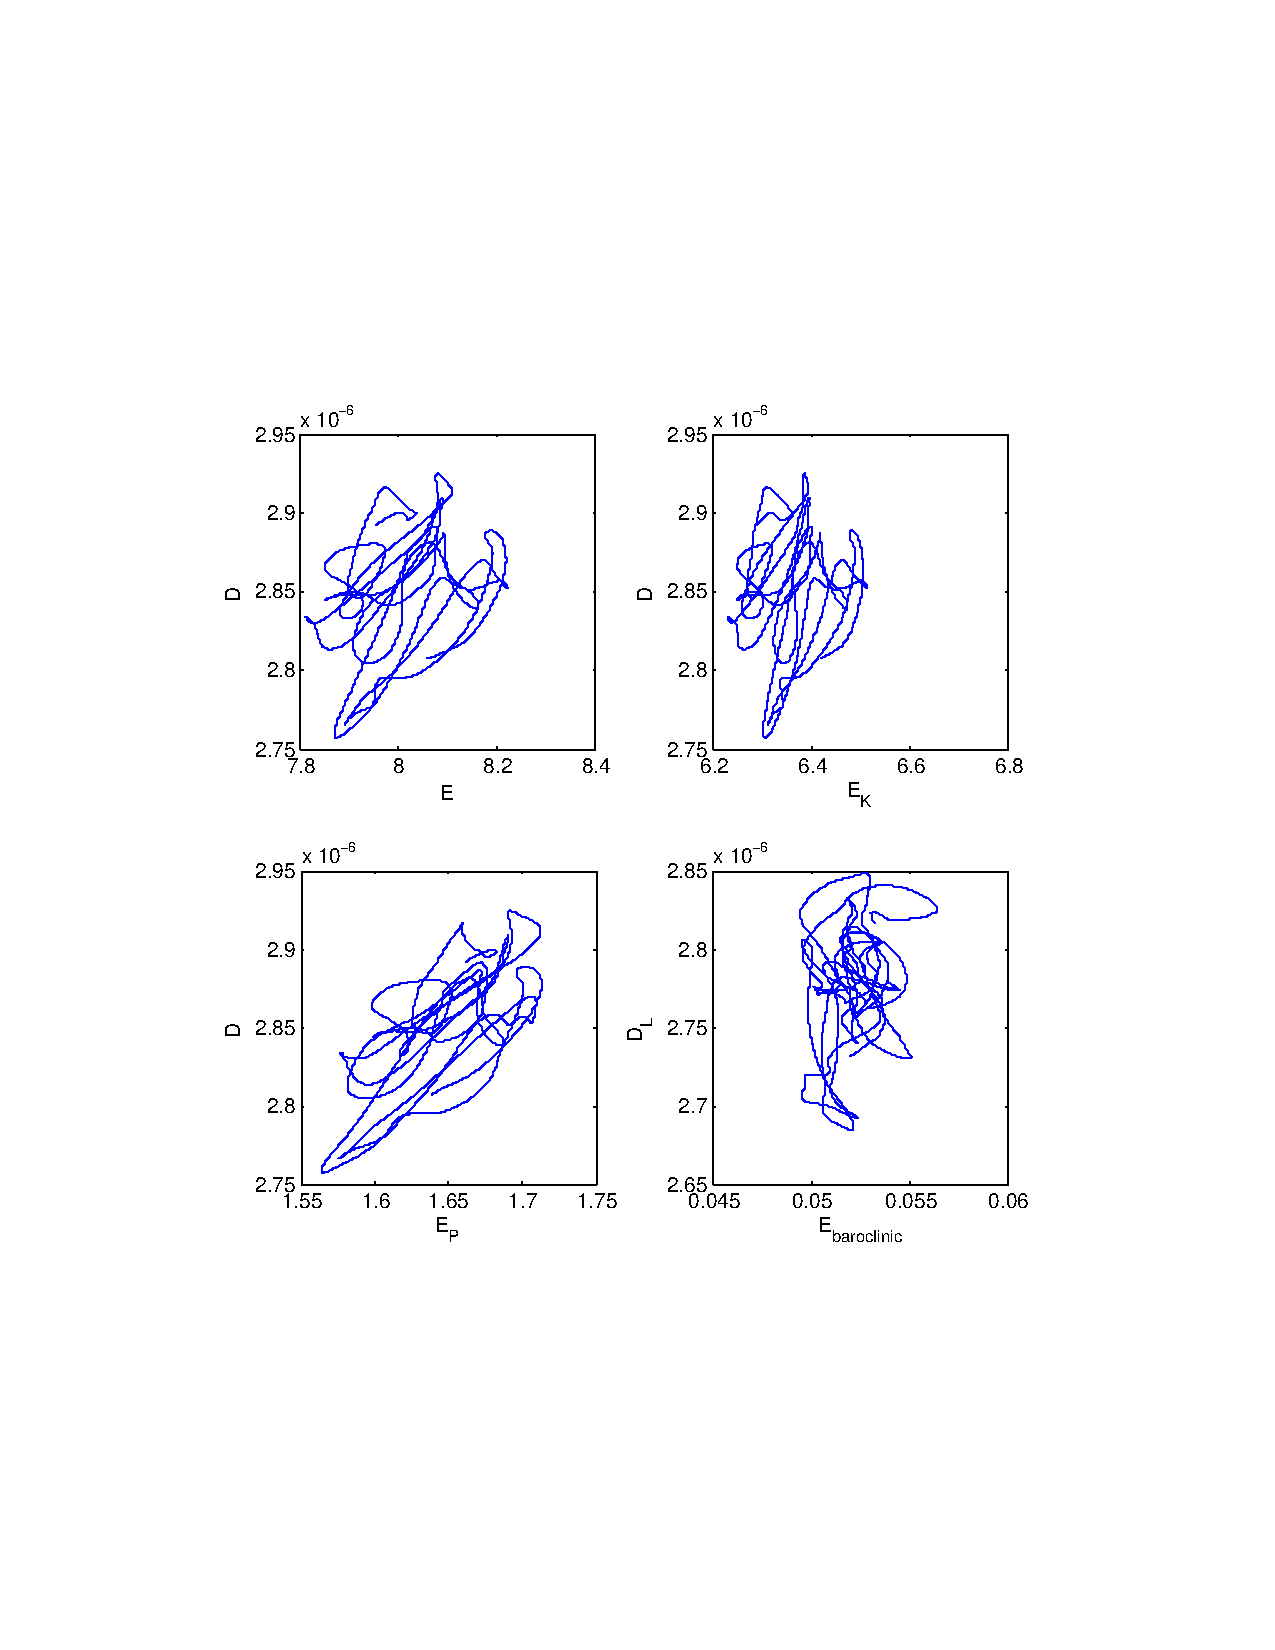
\includegraphics[width=0.95\textwidth]{111023Eplots}
%    & 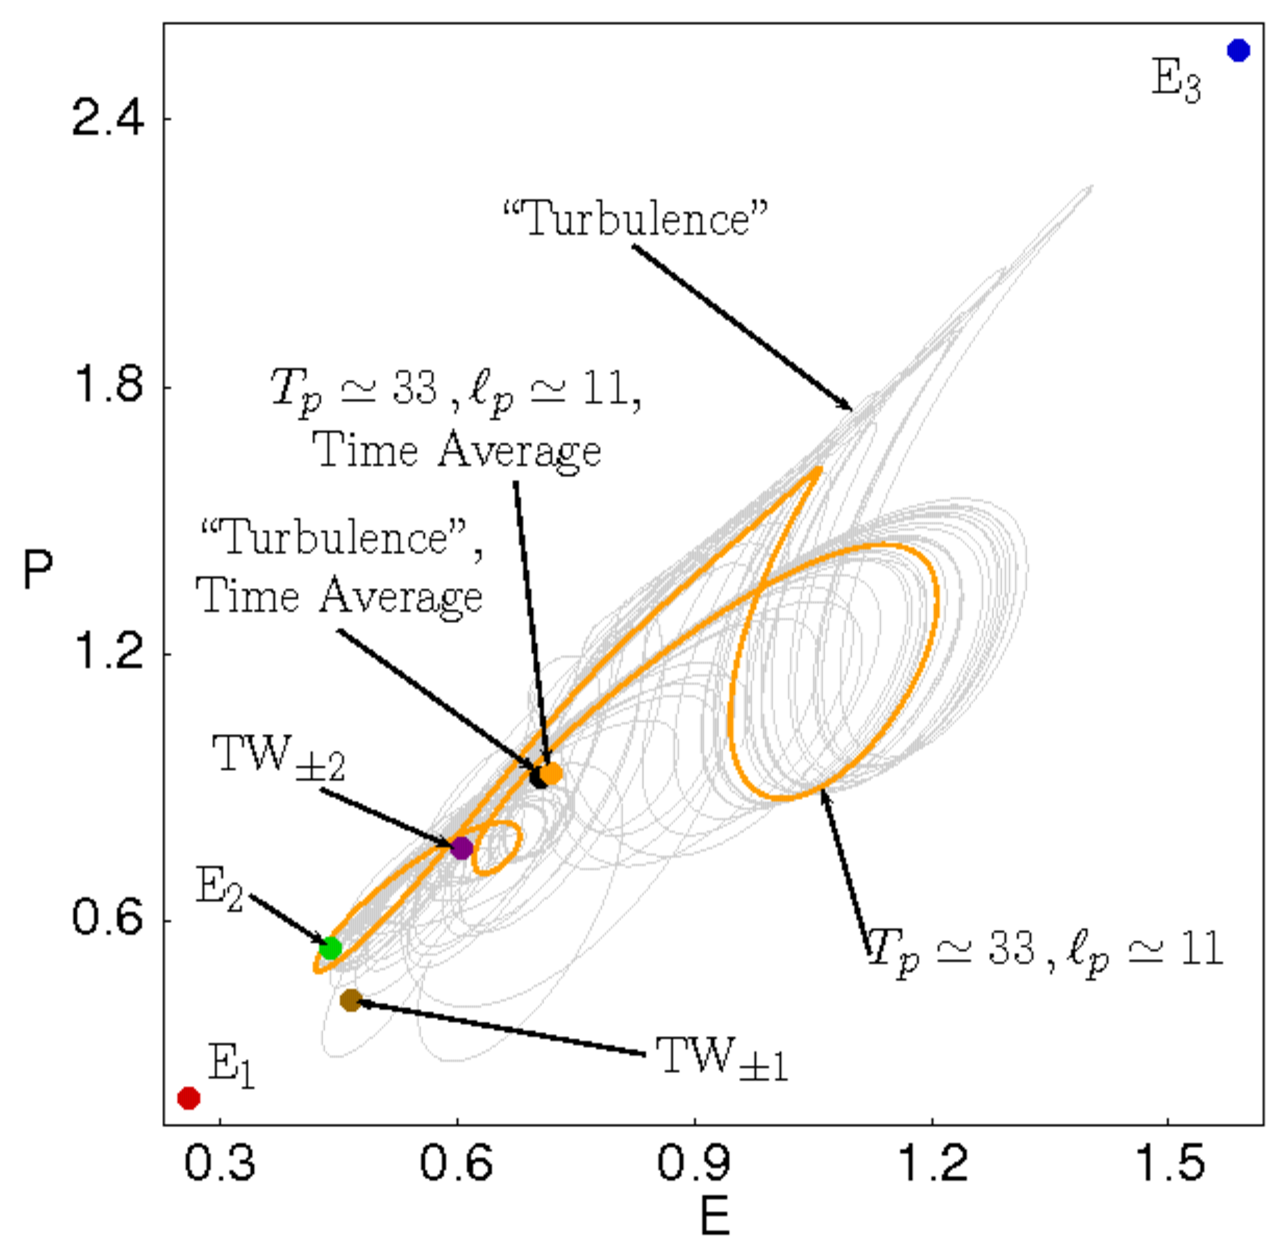
\includegraphics[width=0.46\textwidth, clip=true]{equivaEP_pst}
%  \end{tabular}
\end{center}
\caption{
Energy plots.
See also \reffig{f:111023Ederiv}.
        }
\label{f:111023Eplots}
\end{figure}
%%%%%%%%%%%%%%%%%%%%%%%%%%%%%%%%%%%%%%%%%%%%%%%%%%%%%%%%%%%%%%%%%%%%%


%%%%%%%%%%%%%%%%%%%%%%%%%%%%%%%%%%%%%%%%%%%%%%%%%%%%%%%%%%%%%%%%%%%%%
\begin{figure}%[t]
\begin{center}
% \begin{tabular}{cc}
%        ~~~~~~~~(\textit{a})                        &   ~~~~~~~~(\textit{b}) \\
    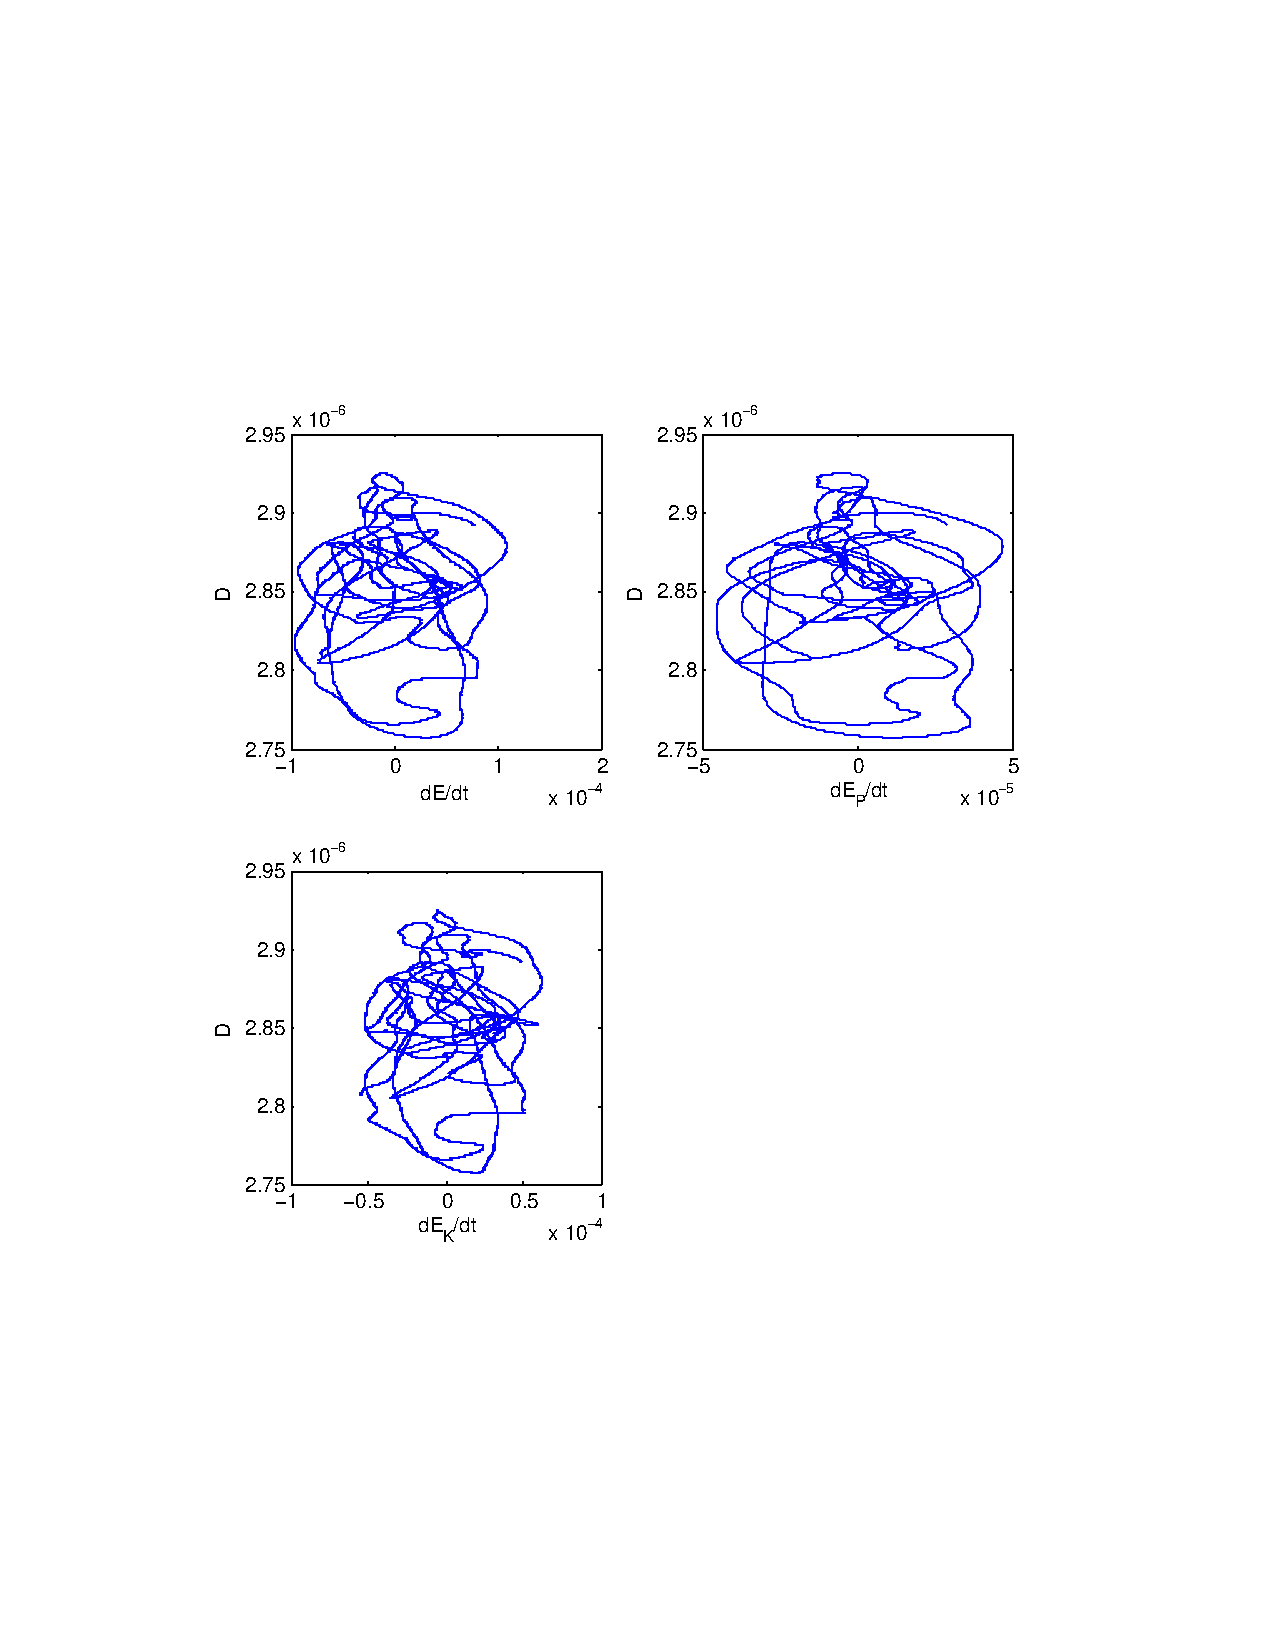
\includegraphics[width=0.95\textwidth]{111023Ederiv}
%    & 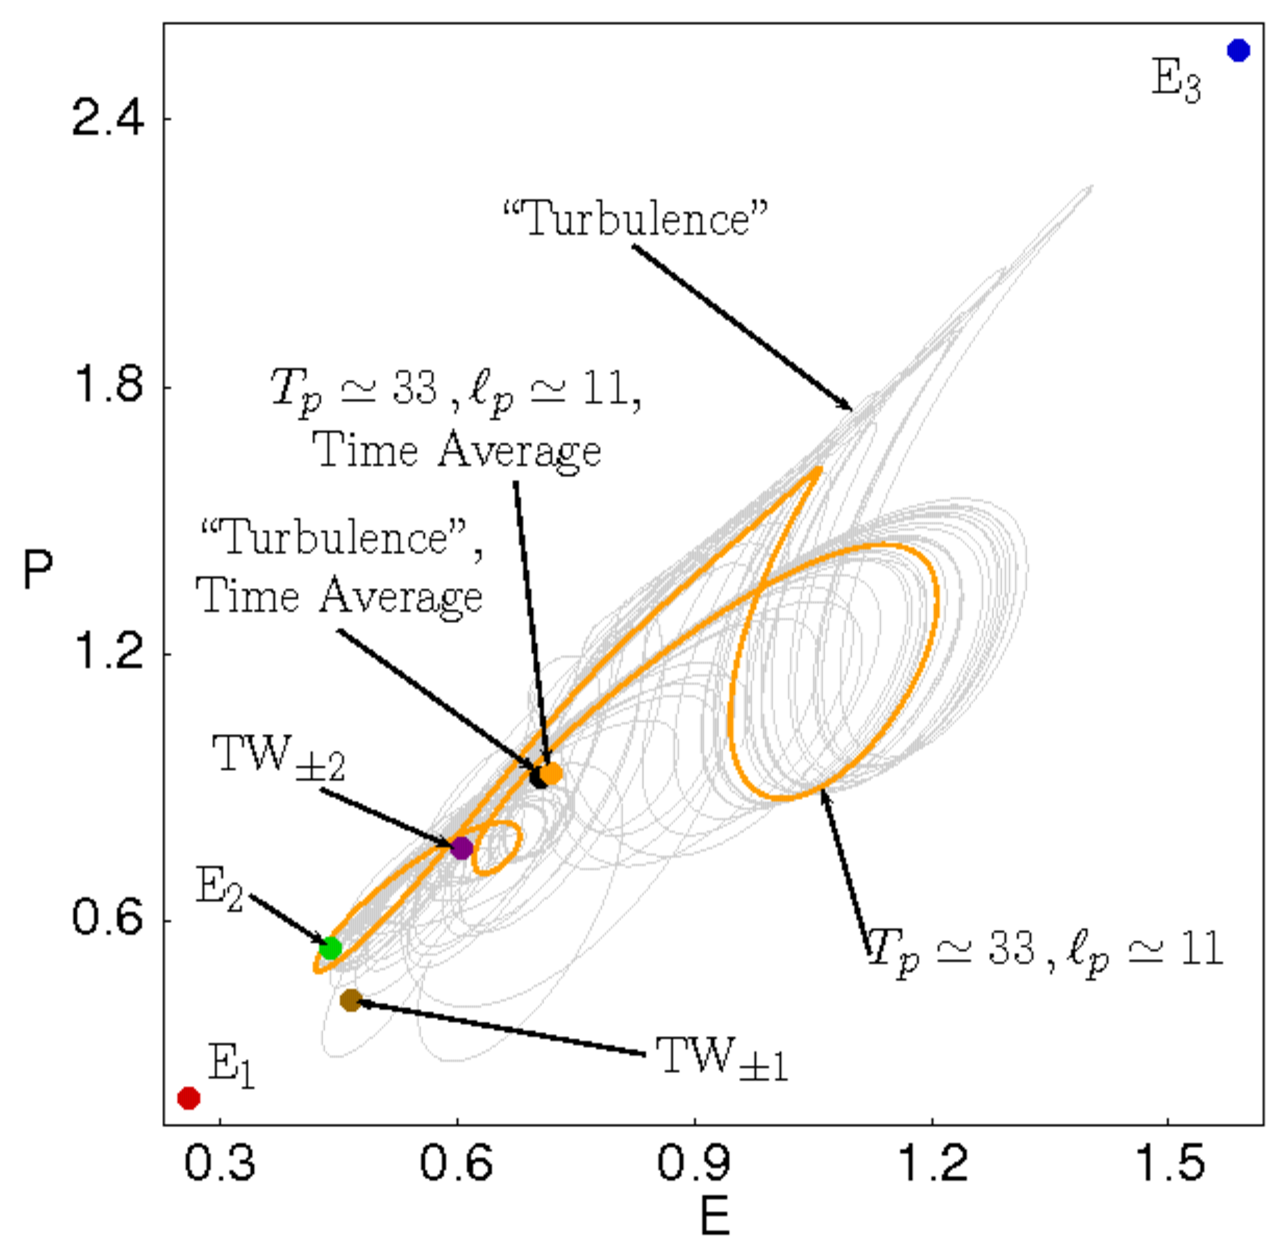
\includegraphics[width=0.46\textwidth, clip=true]{equivaEP_pst}
%  \end{tabular}
\end{center}
\caption{
Energy rates plots.
See also \reffig{f:111023Eplots}.
        }
\label{f:111023Ederiv}
\end{figure}
%%%%%%%%%%%%%%%%%%%%%%%%%%%%%%%%%%%%%%%%%%%%%%%%%%%%%%%%%%%%%%%%%%%%%

\item[2011-11-23 Annalisa]
In \reffig{f:111023Eplots} and \reffig{f:111023Ederiv},
\\
$E_K=$kinetic comp \\
$E_P=$potential \\
$E=$total (sum of the two) \\
$E_{baroclinic}$ is only the baroclinic contribution to the kinetic term
($E_K=E_{barotropic}+E_{baroclinic}$)
$D$ includes large scale contribution from Ekman term and small scale
(newtonian viscosity) from both layers. It is dominated by the large
scale though
The nomenclature for the derivatives is obvious.

I don't see anything that compares too well to the plots you showed me...

\item[2011-12-06 Predrag] In my struggle to avoid dealing with preparing the
AGU talk, I was trying to figure out how to convert Woods Hole prehistoric
FLIC formatted \texttt{vort.fli} into flash, or anything.
\HREF{http://jeff.bovine.net/Fli2Gif}{Fli2Gif} might work in Linux.
Then my friend David clipped it and converted it to 6MB

\texttt{dasbuch/WWW/tutorials/Movies/baroclinVort.flv 1020$\times$900},

\noindent
just like that. Turns out AGU does not allow internet access from the
lecture PCs, so I had to convert my
\HREF{http://ChaosBook.org/tutorials}{ChaosBook.org/tutorials} slides
into PDF. Thankfully, Acrobat allows inclusion of Flash movies - the
result is

\texttt{siminos/talks/AGU11talk.pdf}.

\noindent
It is 38MB, so I have not
added it to svn; ask me if you want a copy.

	
\item[2011-12-12 Francesco Fedele]
I came across the \arXiv{1112.0151} paper on the linear stability of pipe flows for
almost periodic perturbations (with irrational frequency ratios) there is
instability at $\Re \sim 140$..

\item[2012-01-13 Predrag] We should organize this  seminar:
Francesco Fedele\\
Assistant Professor\\
School of Civil \& Environmental Engineering\\
School of Electrical \& Computer Engineering

Title: \emph{From Hamiltonian equations for the ocean dynamics to
traveling waves in Axisymmetric Navier-Stokes Equations}

Abstract:
In this talk I will present an overview of recent results on the
Hamiltonian formulation of envelope equations for the ocean wave dynamics
and experiments for stereo video measurements of oceanic waves off the
Venice coast in Italy. In particular, wave dispersion and energy cascades
observed experimentally confirm that ocean waves can be thought as a
state of weak wave turbulence, i.e. a state of weakly nonlinear
interactions of dispersive elementary waves, the analogue of vortices in
strong Navier-Stokes turbulence. In this regard, I will also discuss a
model reduction of the axisymmetric Navier-Stokes equations for pipe
flows and the existence of traveling waves. In particular, small
perturbations of the laminar flow with amplitude $\eps\approx O(Re^{-2.5})$ obey a
coupled system of nonlinear Korteweg-de Vries type equations, which
support inviscid soliton-type solutions and periodic waves in the form of
toroidal vortex tubes.

\item[2012-02-07 Predrag] Added Sebastian Ortega Arango
<sortega@gatech.edu> project to this blog; enabled svn access, updates
(sortega  baroclinic). See \refchap{chap:OrtegaBlog}.

\item[2012-02-09 Predrag]
Should read
\emph{Hamiltonian description and traveling waves of the spatial Dysthe
 equations}
 \\
by Francesco Fedele and
\HREF{http://www.lama.univ-savoie.fr/~dutykh/}{Denys Dutykh},
\arXiv{1110.3605}.

\item[2012-02-17 Predrag]
Francesco Fedele want us to read Boccotti\rf{Boccotti00}, in particular
\refref{Boccotti11} (I have stored it in CNS Zotero account). Francesco says:
``
a paper on the recurrence of large waves in the ocean ... real data
from experiments in the Mediterranean sea in South Italy .. the sea is
very special there :) .. really .. perfect wind waves all the time ...
experimental site suitable to test theories, etc..

I have another space-time set of data (wave surface in space and time
$\eta(x,y,t)$ over an area of $100^2 m^2$ and duration 1 hour ) collected near
Venice and I would like to check recurrence using Poincar\'e-based
approaches. That would be a good start.
''

\item[2012-06-05 Predrag] Should read
\emph{Effect of differential diffusion and extrapolated Ekman dissipation on
 flux constraints on the two-layer quasi-geostrophic model}
by Eleftherios Gkioulekas,
\arXiv{1206.0315}? He says: ``
 We continue our investigation of an inequality constraining the energy and
potential enstrophy flux spectra in the two-layer quasi-geostrophic model. Its
physical significance is that it can diagnose whether any given model that
allows coexisting downscale cascades of energy and potential enstrophy can
reproduce the Nastr\"om-Gage spectrum, in terms of the total energy spectrum.
This inequality holds unconditionally for two-dimensional turbulence, however
it is far from obvious that it generalizes to multi-layer quasi-geostrophic
models. In previous work we considered the case of a two-layer
quasi-geostrophic model in which the dissipation terms for each layer are
dependent only on the streamfunction field of the corresponding layer. We now
generalize this configuration as follows: First, following a 1980 paper by
Salmon, we use an extrapolated Ekman term at the bottom layer which uses the
streamfunction field of both layers to approximate the streamfunction field at
the surface boundary layer. Second, for reasons explained in detail in the
paper itself, we use small-scale dissipation terms with different
hyperviscosity coefficients. Sufficient conditions for satisfying the flux
inequality are given under this more general dissipation configuration, and we
discuss the potential role of extrapolated Ekman dissipation and differential
small-scale dissipation in violating the flux inequality. ''

\item[2012-06-05 Annalisa] I just turned down the invitation from JFM to
review that manuscript because I'm leaving for the cruise in the gulf
tomorrow... not sure is relevant (and pleased I turned down the
review, now that I see the full manuscript...)

\end{description}
